% !TeX program = pdflatex
% Notes for Ordinary Differential Equations (LaTeX edition)
% Transcribed from the handwritten BOOX notebook (84 pages, Oct 2026).
% Figures are redrawn in TikZ (see the accompanying fig sources).
\documentclass[11pt]{article}
\usepackage[a4paper,margin=2.3cm]{geometry}
\usepackage{amsmath,amssymb,amsthm,mathtools}
\usepackage{graphicx}
\usepackage{booktabs}
\usepackage{tikz}
\usetikzlibrary{arrows.meta,calc,decorations.pathmorphing,decorations.markings,patterns,positioning}
\usepackage[colorlinks=true,linkcolor=blue!55!black,urlcolor=blue!55!black,citecolor=blue!55!black]{hyperref}

\setcounter{secnumdepth}{-2}
\setcounter{tocdepth}{1}

\theoremstyle{definition}
\newtheorem*{definition}{Def}
\newtheorem*{proposition}{Prop}
\newtheorem*{theorem}{Thm}
\newtheorem*{lemma}{Lemma}
\newtheorem*{corollary}{Cor}
\newtheorem*{example}{Eg}
\newtheorem*{exercise}{Ex}
\newtheorem*{remark}{Rem}
\newtheorem*{question}{Q}
\theoremstyle{remark}

\newcommand{\R}{\mathbb{R}}
\newcommand{\Z}{\mathbb{Z}}
\newcommand{\N}{\mathbb{N}}
\newcommand{\CC}{\mathbb{C}}
\newcommand{\tr}{\operatorname{tr}}
\newcommand{\real}{\operatorname{Re}}
\newcommand{\imag}{\operatorname{Im}}
\newcommand{\diag}{\operatorname{diag}}
\newcommand{\Ker}{\operatorname{Ker}}
\newcommand{\W}{\operatorname{W}}

% Chapter / section headings (manual numbering, matching the notebook)
\newcommand{\chap}[1]{%
  \clearpage
  \vspace*{0.4em}
  {\centering\Large\bfseries #1\par}
  \vspace{0.5em}
  \addcontentsline{toc}{section}{#1}}
\newcommand{\secn}[1]{\subsection*{#1}\addcontentsline{toc}{subsection}{#1}}
\newcommand{\subsecn}[1]{\subsubsection*{#1}}

\graphicspath{{figs/}}

\title{\bfseries Ordinary Differential Equations\\[0.3em]\large Lecture Notes (LaTeX edition)}
\author{}
\date{October 2026}

\begin{document}
\maketitle
\vspace{-3em}

\begin{abstract}
\noindent
These notes are transcribed from my handwritten notebook on Ordinary Differential Equations.
They cover: explicit solution methods for first order ODEs (exact equations, separating variables,
integrating factors, implicit equations); existence, uniqueness and extension of solutions
(Gronwall, Arzel\`a--Ascoli, Picard--Lindel\"of, Peano, Osgood, comparison principles, dependence
on data and parameters); linear systems (fundamental matrices, constant coefficients, higher order
equations, Floquet theory); the power series method (Cauchy theory, Frobenius theory, Bessel
functions); and Sturm--Liouville theory (separation and comparison theorems, the regular and
periodic Sturm--Liouville problems, boundary value problems for nonlinear ODEs).
\end{abstract}

\tableofcontents

%======================================================================
\chap{Chapter 1\quad Introduction}

\secn{1.1\quad What is an ODE}

\begin{definition}[(ODE)]
$F$ is a given function, $x\in\R$, $y(x)\colon I\subseteq\R\to V\subseteq\R^m$ $(m<\infty)$.
An ODE is
\[
F(x, y(x), y'(x), \dots, y^{(n)}(x)) = 0,
\]
which has order $n$.
\end{definition}

\begin{definition}[(Classical solution)]
$\varphi(x)\colon J\subseteq\R\to V$, $\varphi\in D^n(J)$, s.t.
\[
F(x, \varphi(x), \varphi'(x), \dots, \varphi^{(n)}(x)) = 0, \quad \forall x\in J.
\]
\end{definition}

\begin{remark}
If $F$ is good enough, by implicit function theorem,
\[
y^{(n)} = f(x, y, y', \dots, y^{(n-1)}).
\]
\end{remark}

\textbf{Notes for example 1.5:} long time behavior.

\begin{center}
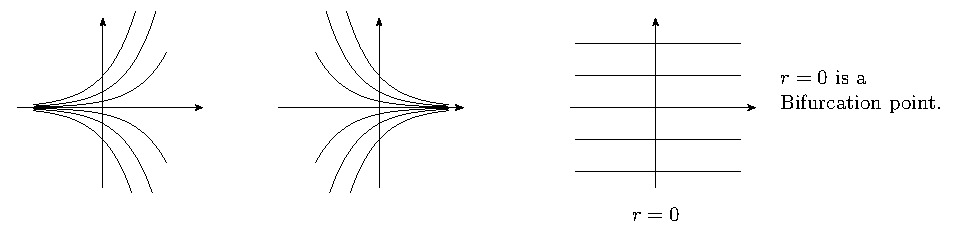
\includegraphics[scale=0.62]{ch01_fig_1_1_1}
\end{center}

$r=0$ is a \textbf{bifurcation point}.

\begin{definition}[(General solution)]
For $F(x, y, y', \dots, y^{(n)}) = 0$, if $\varphi(x, C_1, \dots, C_n)$ solves it, and $C_i$ are
\textbf{independent parameters}, we say $\varphi$ is a general solution.

Here, ``independent parameters'' means
\[
\det\frac{\partial(\varphi, \varphi', \dots, \varphi^{(n-1)})}{\partial(C_1, C_2, \dots, C_n)} \neq 0.
\]
\end{definition}

\begin{remark}
If $\varphi$ is a general solution, then given any initial data
$(y(0), y'(0), \dots, y^{(n-1)}(0)) = (a_0, a_1, \dots, a_{n-1})$,
we can always find some $C_i$ s.t. $\varphi(x, C_1, \dots, C_n)$ solves the IVP.
This is true by the inverse function theorem.
\end{remark}

\secn{1.2\quad Find explicit solutions for ODE}

\subsecn{1.2.1\quad Exact equation}

Consider $P(x,y)\,dx + Q(x,y)\,dy = 0$.

\begin{definition}[(general integral)]
If $\exists\ \Phi(x,y)\in C^1$ s.t.
\[
d\Phi = P(x,y)\,dx + Q(x,y)\,dy,
\]
then the equation is called an \textbf{exact equation}, and $\Phi$ is called a general integral of
the equation. Its solutions are given by $\Phi(x,y) = C$.
\end{definition}

\begin{lemma}[(Exact-equation lemma; proof see the lecture notes)]
Assume $P$, $Q$ and $\partial P/\partial y$, $\partial Q/\partial x$ are continuous in a simply
connected domain. Then the equation is exact iff
\[
\frac{\partial P}{\partial y} = \frac{\partial Q}{\partial x}.
\]
In this case,
\[
\Phi(x,y) = \int_{x_0}^{x} P(s,y)\,ds + \int_{y_0}^{y} Q(x,\theta)\,d\theta + C.
\]
\end{lemma}

\begin{remark}
Compare with: ``$\int_\gamma P\,dx + Q\,dy$ is independent of path iff
$\frac{\partial P}{\partial y} = \frac{\partial Q}{\partial x}$ (for a simply connected domain).''
\end{remark}

\subsecn{1.2.2\quad Separating variables}

If $P(x,y) = X(x)Y(y)$, $Q(x,y) = X_1(x)Y_1(y)$, then we rewrite
\[
\frac{X(x)}{X_1(x)}\,dx + \frac{Y_1(y)}{Y(y)}\,dy = 0,
\]
which is obviously exact. Notice $X_1(x) = 0$ (i.e. $x = a_1$) or $Y_1(y) = 0$ (i.e. $y = b_1$),
which are also solutions.

\begin{example}[(Logistic population model)]
$\frac{dy}{dt} = ry(N-y)$
\[
\Rightarrow\ \frac{dy}{y(N-y)} = r\,dt \quad (\text{or } y\equiv 0,\ y\equiv N)
\ \Rightarrow\ \frac{y}{N-y} = k\,e^{Nrt}\quad (k\in\R)
\]
\[
\Rightarrow\ y(t) = \frac{Nke^{Nrt}}{1+ke^{Nrt}} = N - \frac{N(N-y(0))}{(N-y(0)) + y(0)\,e^{Nrt}}.
\]
\end{example}

\begin{center}
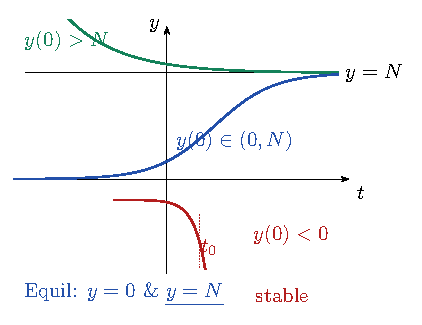
\includegraphics[scale=0.6]{ch01_fig_1_2_1}
\end{center}

Equilibrium: $y = 0$ \& $y = N$ (stable).

\begin{example}
$(x^2+1)(y^2-1)\,dx + xy\,dy = 0$
\[
\Rightarrow\ y^2 - 1 = \frac{k}{x^2 e^x}\quad (k\in\R), \qquad\&\quad x \equiv 0.
\]
\end{example}

\begin{center}
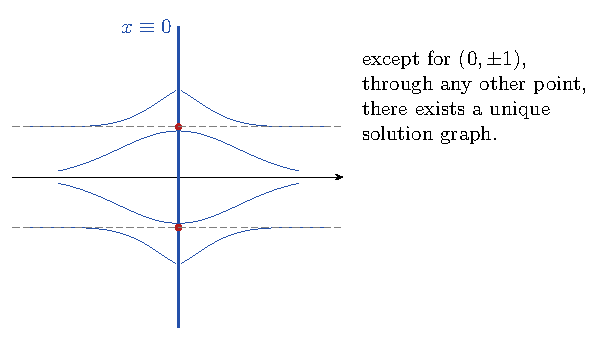
\includegraphics[scale=0.62]{ch01_fig_1_2_2}
\end{center}

Except for $(0,\pm 1)$, through any other point there exists a unique solution graph.

\begin{example}
$y' = \frac{3}{2}y^{1/3}$
\[
\Rightarrow\ y^2 = (x+C)^3 \quad \& \quad y \equiv 0.
\]
\end{example}

\begin{center}
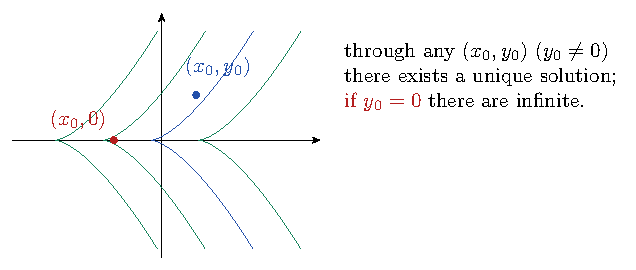
\includegraphics[scale=0.6]{ch01_fig_1_2_3}
\end{center}

Through any $(x_0, y_0)$ with $y_0 \neq 0$ there exists a unique solution; if $y_0 = 0$ there are
infinitely many.

\begin{example}[(Homogeneous equation of order $n$)]
We call $f(x,y)$ a homogeneous function of order $n$ if $f(tx, ty) = t^n f(x,y)$ for all $t$.

Consider $M(x,y)\,dx + N(x,y)\,dy = 0$, in which $M$, $N$ are homogeneous of order $n$.
Set $y = ux$. Then $M(x,y) = x^n M(1,u)$, $dy = x\,du + u\,dx$,
\[
x^n\bigl(M(1,u) + uN(1,u)\bigr)\,dx + x^{n+1}N(1,u)\,du = 0.
\]
\end{example}

\begin{example}
$\frac{dy}{dx} = \frac{x+y}{x-y}$. Set $y = ux$, $dy = u\,dx + x\,du$:
\[
\frac{u\,dx + x\,du}{dx} = \frac{x+ux}{x-ux} = \frac{1+u}{1-u}
\ \Rightarrow\ \frac{(1-u)\,du}{1+u^2} = \frac{dx}{x}
\]
(here, check that $x\equiv 0$ is not a solution)
\[
\Rightarrow\ \arctan u - \tfrac{1}{2}\ln(1+u^2) = \ln|x| + C.
\]
\end{example}

\subsecn{1.2.3\quad Integrating factor}

Find a function $a(x,y)$ s.t. $aP(x,y)\,dx + aQ(x,y)\,dy = 0$ is exact. Then $\exists\ \Phi$ s.t.
$d\Phi = aP\,dx + aQ\,dy$,
\[
\frac{\partial(aP)}{\partial y} = \frac{\partial^2\Phi}{\partial x\,\partial y} = \frac{\partial(aQ)}{\partial x}.
\]

\begin{lemma}
$P\,dx + Q\,dy = 0$ admits an integrating factor of the form $a(x)$ iff
$G = \bigl(\frac{\partial P}{\partial y} - \frac{\partial Q}{\partial x}\bigr)/Q$ is independent
of $y$; in this case $a(x) = e^{\int_{x_0}^{x} G(t)\,dt}$.

Similarly, it admits an integrating factor of the form $a(y)$ iff
$H = \bigl(\frac{\partial Q}{\partial x} - \frac{\partial P}{\partial y}\bigr)/P$ is independent
of $x$; in this case $a(y) = e^{\int_{y_0}^{y} H(t)\,dt}$ is an integrating factor.
\end{lemma}

\begin{example}
$(3x^2y + 2xy + y^3)\,dx + (x^2 + y^2)\,dy = 0$:
\[
\frac{\partial P}{\partial y} = 3x^2 + 2x + 3y^2, \qquad
\frac{\partial Q}{\partial x} = 2x, \qquad
\frac{\frac{\partial P}{\partial y} - \frac{\partial Q}{\partial x}}{Q} = 3.
\]
Take $e^{3x}$ as the integrating factor.
\end{example}

\begin{example}[Back to the homogeneous equation]
\[
x^n\bigl(M(1,u) + uN(1,u)\bigr)\,dx + x^{n+1}N(1,u)\,du = 0.
\]
Notice $\dfrac{1}{x^{n+1}(M(1,u) + uN(1,u))} = \dfrac{1}{xM(x,y) + yN(x,y)}$; we guess this is an
integrating factor, i.e.\ $\dfrac{M}{xM+yN}\,dx + \dfrac{N}{xM+yN}\,dy$ is exact.

\textbf{Pf.}\ $\partial_y\Bigl(\dfrac{M}{xM+yN}\Bigr) - \partial_x\Bigl(\dfrac{N}{xM+yN}\Bigr)
= \frac{1}{(xM+yN)^2}\Bigl[N(xM_x + yM_y) - M(xN_x + yN_y)\Bigr] = 0.$ \qed
\end{example}

\subsecn{1.2.4\quad First order equation}

Consider $\frac{dy}{dx} + p(x)y - q(x) = 0$, i.e.
\begin{equation}
\bigl(p(x)y - q(x)\bigr)\,dx + dy = 0. \tag{$*$}
\end{equation}
Taking the integrating factor $a(x) = e^{\int_{x_0}^{x} p(s)\,ds}$,
\[
e^{\int_{x_0}^{x} p(s)\,ds}\bigl(p(x)y - q(x)\bigr)\,dx + e^{\int_{x_0}^{x} p(s)\,ds}\,dy = 0
\ \Rightarrow\ e^{\int_{x_0}^{x} p(s)\,ds}\cdot y - \int_{x_0}^{x} e^{\int_{x_0}^{t} p(s)\,ds}\,q(t)\,dt = C,
\]
\[
\Rightarrow\ y = e^{-\int_{x_0}^{x} p(s)\,ds}\Bigl(C + \int_{x_0}^{x} q(t)\,e^{\int_{x_0}^{t} p(s)\,ds}\,dt\Bigr).
\]

\begin{proposition}
Every $y(x)$ solving $(*)$ takes the form above.

\textbf{Pf.}\ $\Bigl(y(x)e^{\int_{x_0}^{x} p(s)\,ds}\Bigr)' = e^{\int_{x_0}^{x} p(s)\,ds}(y'(x) + p(x)y(x)) = e^{\int_{x_0}^{x} p(s)\,ds}\,q(x)$. \qed
\end{proposition}

\begin{lemma}
(1) For the homogeneous equation $y' + p(x)y = 0$, the solutions form a 1-dim vector space.

(2) For the inhomogeneous equation, the general solution consists of two parts: one is the general
solution of the homogeneous equation, the other is a special solution.

(3) The first order equation has a unique solution for the IVP.
\end{lemma}

\begin{example}
$\frac{dy}{dx} + ay = f(x)$, where $f(x+2\pi) = f(x)$, $x\in\R$. Find a $2\pi$-periodic solution.

\textbf{Sol.} Claim: if we have a solution s.t.\ $y(0) = y(2\pi)$, then $y(x)$ is $2\pi$-periodic.
Indeed $y(x)$ is a solution $\Rightarrow y(x+2\pi)$ is also a solution; then
$z(x) = y(x+2\pi) - y(x)$ solves $z' + az = 0$ (from the lemma), so $z(x) = e^{-ax}z(0)$; if
$y(0) = y(2\pi)$ then $z(0) = 0 \Rightarrow z(x)\equiv 0 \Rightarrow y(x+2\pi) = y(x)$ for all $x$.

So we just solve the equation and impose $y(0) = y(2\pi)$:
\[
y' = -ay + f(x) \ \Rightarrow\ y = e^{-ax}\Bigl(C + \int_0^x f(s)\,e^{as}\,ds\Bigr),
\]
\[
y(0) = y(2\pi) \ \Rightarrow\ C = \frac{e^{-2\pi a}\int_0^{2\pi} f(x)\,e^{ax}\,dx}{1 - e^{-2\pi a}}.
\]
\end{example}

\subsecn{1.2.5\quad First order ODE in implicit form}

Consider $F(x, y', y) = 0$. \hfill $(*)$

\textbf{Special case.} If $y$ can be solved: $y = f(x, y')$; let $p := \frac{dy}{dx}$. Then
\[
p = \frac{dy}{dx} = \frac{\partial f}{\partial x} + \frac{\partial f}{\partial p}\cdot\frac{dp}{dx}
\ \Rightarrow\ \frac{\partial f}{\partial p}(x,p)\,\frac{dp}{dx} = p - \frac{\partial f}{\partial x}(x,p).
\]
If $p = p(x)$ is a solution, then $f(x, p(x))$ solves $(*)$.

\begin{example}[(Clairaut equation)]
$y = xp + f(p)$, $p := \frac{dy}{dx}$:
\[
\frac{dy}{dx} = p + x\frac{dp}{dx} + f'(p)\frac{dp}{dx}
\ \Rightarrow\ \bigl(x + f'(p)\bigr)\frac{dp}{dx} = 0,
\]
\[
\Rightarrow\ y = cx + f(c) \quad\text{or}\quad
\begin{cases} x = -f'(p) \\ y = -f'(p)\,p + f(p) \end{cases}
\quad (p \text{ as a parameter}).
\]
\end{example}

\textbf{Method of parameter.} $F(x, y, p) = 0$: take $x = x(u,v)$, $y = y(u,v)$, $p = p(u,v)$.

\begin{example}
$x = (y')^3 + y'$. See $p = y'$ as a parameter:
\[
x = p^3 + p, \qquad dy = p\,dx = p(3p^2+1)\,dp
\ \Rightarrow\ \begin{cases} x = p^3 + p \\ y = \frac{3}{4}p^4 + \frac{1}{2}p^2 + C. \end{cases}
\]
\end{example}

\subsecn{1.2.6\quad Other examples}

\begin{example}
$\frac{dy}{dx} = f(x+y)$: let $z = x + y(x)$, then $\frac{dz}{dx} = 1 + \frac{dy}{dx} = f(z)$.
\end{example}

\begin{example}
$\frac{dy}{dx} = f\Bigl(\frac{ax+by+c}{mx+ky+l}\Bigr)$.

Case 1. $c = 0$, $l = 0$: the equation is homogeneous of order 0.

Case 2. $c\,l \neq 0$, $\Delta = \begin{vmatrix} a & b \\ m & k \end{vmatrix} \neq 0$: then
$\exists\ \tilde{x} = x + x_0$, $\tilde{y} = y + y_0$ s.t.
$\frac{d\tilde{y}}{d\tilde{x}} = f\Bigl(\frac{a\tilde{x} + b\tilde{y}}{m\tilde{x} + k\tilde{y}}\Bigr)$.

Case 3. $c\,l \neq 0$, $\Delta = 0$: then
$f\Bigl(\frac{ax+by+c}{mx+ky+l}\Bigr) = f\Bigl(\frac{ax+by+c}{\lambda(ax+by)+l}\Bigr)$;
taking $z = ax + by$ we can separate variables.
\end{example}

\begin{example}[(Bernoulli eq.)]
$\frac{dy}{dx} + p(x)y = q(x)y^n$
\[
\Rightarrow\ \frac{1}{y^n}\frac{dy}{dx} + p(x)y^{1-n} = q(x);
\qquad z = y^{1-n}(x) \ \Rightarrow\ \frac{dz}{dx} = (1-n)\bigl(q(x) - p(x)z\bigr),
\]
a first order equation for $z(x)$.
\end{example}

\begin{example}[(Riccati eq.)]
$\frac{dy}{dx} = a(x)y^2 + b(x)y + c(x)$.

\begin{lemma}
(1) If $\Phi(x)$ is a solution, then we can find all solutions.

\textbf{Pf.}\ Assume $y(x) = \Phi(x) + u(x)$:
\[
y' = \Phi'(x) + u'(x) = a(\Phi+u)^2 + b(\Phi+u) + c = \Phi' + 2a\Phi u + au^2 + bu,
\]
\[
\Rightarrow\ \frac{du}{dx} = (2a\Phi + b)u + au^2 \qquad \text{(Bernoulli eq.)}
\]

(2) If $\varphi_1, \varphi_2$ are two given solutions, then any solution $y(x)$ satisfies
\[
\frac{y-\varphi_1}{y-\varphi_2} = C\exp\Bigl(\int_{x_0}^{x} a(s)(\varphi_1-\varphi_2)(s)\,ds\Bigr).
\]

(3) If $\varphi_1, \varphi_2, \varphi_3$ are solutions, then
\[
\frac{y-\varphi_1}{y-\varphi_2}\Big/\frac{\varphi_3-\varphi_1}{\varphi_3-\varphi_2} = C.
\]
\end{lemma}
\end{example}

\begin{theorem}[(Bernoulli \& Liouville)]
$\frac{dy}{dx} = ay^2 + bx^m$ $(a,b,m\in\R,\ a\neq 0)$ can be solved iff
\[
m = 0,\quad -2,\quad \frac{-4k}{2k+1},\quad \frac{-4k}{2k-1}\quad (k\in\Z).
\]
\end{theorem}

%======================================================================
\chap{Chapter 2\quad Existence \& Uniqueness}

\secn{2.1\quad Preparation}

\subsecn{2.1.1\quad Gronwall inequality}

\begin{lemma}[Version 1]
$f\in C^1[a,b]$, $g\in C[a,b]$, and $f' \le gf$ for all $x\in[a,b]$. Then
\[
f(x) \le f(x_0)\exp\Bigl(\int_{x_0}^{x} g(s)\,ds\Bigr), \qquad \forall\, x\ge x_0,\ x_0\in[a,b].
\]
\textbf{Pf.}\ $\bigl(e^{-\int_{x_0}^{x} g(s)\,ds}f\bigr)' = e^{-\int_{x_0}^{x} g(s)\,ds}(f' - gf) \le 0$;
then $e^{-\int_{x_0}^{x} g(s)\,ds}f(x) \le f(x_0)$. \qed
\end{lemma}

\begin{lemma}[Version 2]
$f\in C^1[a,b]$, $g, h\in C[a,b]$, $f' \le h + gf$. Then
\[
f(x) \le e^{\int_{x_0}^{x} g(s)\,ds}\Bigl(f(x_0) + \int_{x_0}^{x} e^{-\int_{x_0}^{t} g(s)\,ds}\,h(t)\,dt\Bigr),
\qquad \forall\, x\ge x_0.
\]
\textbf{Pf.}\ $\bigl(e^{-\int_{x_0}^{x} g(s)\,ds}f(x)\bigr)' \le e^{-\int_{x_0}^{x} g(s)\,ds}\,h(x)$;
then apply Version 1. \qed
\end{lemma}

\begin{lemma}[Version 3]
$f, g\in C[a,b]$, $g\ge 0$, $f(x) \le C + \int_a^x g(s)f(s)\,ds$. Then
$f(x) \le C\exp\bigl(\int_a^x g(s)\,ds\bigr)$.

\textbf{Pf.}\ $\Phi(x) := C + \int_a^x g(s)f(s)\,ds$, $\Phi'(x) = g(x)f(x) \le g(x)\Phi(x)$;
$\Rightarrow f(x) \le \Phi(x) \overset{\text{Ver 1}}{\le} C\exp\bigl(\int_a^x g(s)\,ds\bigr)$. \qed
\end{lemma}

\begin{lemma}[Version 4]
$f, g, h\in C[a,b]$, $g\ge 0$, $f(x) \le h(x) + \int_a^x g(s)f(s)\,ds$. Then
\[
f(x) \le h(x) + e^{\int_a^x g(s)\,ds}\Bigl[\int_{x_0}^{x} e^{-\int_{x_0}^{t} g(s)\,ds}\,g(t)\,h(t)\,dt\Bigr].
\]
\textbf{Pf.}\ $\Phi(x) := \int_a^x g(s)f(s)\,ds$, $\Phi' = gf \le g(h+\Phi) = gh + g\Phi$;
$\Rightarrow f(x) \le h(x) + \Phi(x) \overset{\text{Ver 2}}{\le} \ldots$ \qed
\end{lemma}

\subsecn{2.1.2\quad Ascoli--Arzel\`a lemma}

\begin{definition}
$f_n\in C[a,b]$ are called \textbf{uniformly bounded} if $|f_n(x)| < K$ for all $x, n$.
\end{definition}

\begin{definition}
$f_n\in C[a,b]$ are called \textbf{equicontinuous} if $\forall\varepsilon > 0\ \exists\,\delta$ s.t.\
$|x-y| < \delta \Rightarrow |f_n(x) - f_n(y)| < \varepsilon$ for all $n$.
\end{definition}

\begin{lemma}[(Arzel\`a--Ascoli)]
If $f_n\in C[0,1]$ are uniformly bounded \& equicontinuous, then $\exists$ a subsequence
$f_{n_j} \Rightarrow f\in C[a,b]$.

\textbf{Pf.}\ Let $\{x_n\} := \mathbb{Q}\cap[a,b]$. For $x_1$, $\{f_n(x_1)\}$ is bounded, so there is
a subsequence $f_{1,n}(x_1)$ converging. For $x_2$: $\{f_{1,n}(x_2)\}$ is bounded, take a further
subsequence $\{f_{2,n}(x_2)\} \subseteq \{f_{1,n}(x_2)\}$ converging. Repeating the process gives
$\{f_{k,n}\} \subseteq \{f_{l,n}\}$ for $l \le k-1$. Take the diagonal $\{f_{n,n}\}$: $f_{n,n}(x_j)$
converges for every rational $x_j$.

Since $\{f_n\}$ is equicontinuous, $\forall\varepsilon>0\ \exists\delta>0$:
$|x-y|<\delta \Rightarrow |f_n(x)-f_n(y)| < \varepsilon/3$. Cover $[a,b] \subseteq \bigcup_{k=1}^{K} B(x_{j_k}, \delta)$;
$\forall\varepsilon>0\ \exists\, N = N(\varepsilon, j_k)$ s.t.\
$|f_{n,n}(x_{j_k}) - f_{m,m}(x_{j_k})| < \varepsilon$. Take $N_0 = \max_k N(\varepsilon, j_k)$; then for
$n, m > N_0$:
\[
|f_{n,n}(x) - f_{m,m}(x)|
= |f_{n,n}(x) - f_{n,n}(x_j)| + |f_{n,n}(x_j) - f_{m,m}(x_j)| + |f_{m,m}(x_j) - f_{m,m}(x)| < \varepsilon.
\]
Hence $f_{n,n}$ converges uniformly. \qed
\end{lemma}

\begin{remark}
If $M$ is a compact set of $\R^n$, the A--A thm.\ applies to $\{f_n\} \subseteq C(M, \R)$. Also, the
A--A thm applies to $C(X,Y)$ where $X, Y$ are complete metric spaces, $X$ compact and $\{f_n\}$
totally bounded.
\end{remark}

\secn{2.2\quad Picard--Lindel\"of thm.}

Consider the IVP
\[
\begin{cases} \dfrac{dy}{dx} = f(x,y) \\ y(x_0) = y_0 \end{cases}
\qquad D = \bigl\{(x,y)\in\R^2 :\ |x-x_0|<a,\ |y-y_0|<b\bigr\}.
\]

\begin{definition}[(Lipschitz)]
$f$ is called $y$-Lipschitz on $D$ if $|f(x,y_1) - f(x,y_2)| < L\,|y_1 - y_2|$ for all
$(x,y_1), (x,y_2)\in D$. $f$ is called locally Lipschitz on $\Omega$ if every $(x_0,y_0)\in\Omega$
has a neighborhood $D$ s.t.\ $f$ is Lipschitz on $D$.
\end{definition}

\begin{theorem}[(Picard--Lindel\"of)]
If $f \in C(D)$ and $f$ is $y$-Lipschitz on $D$, then the Cauchy problem has a unique solution
$y(x)$ on $[x_0 - h,\ x_0 + h]$, where $h := \min\{a,\ b/M\}$.
\end{theorem}

\textbf{Pf.}
\textbf{Step 1.} Transform to the integral equation
\begin{equation}
y(x) = y_0 + \int_{x_0}^{x} f(s, y(s))\, ds. \tag{$*$}
\end{equation}
We claim ODE $\iff$ $(*)$: if $y \in C^1$ solves the ODE then $y$ satisfies $(*)$; if $y \in C$
satisfies $(*)$ then $y \in C^1$ \& solves the ODE. Denote
$\Phi(y) := y_0 + \int_{x_0}^{x} f(s, y(s))\, ds$; we search for a fixed point $y = \Phi(y)$.
(Formally we can use the Banach thm.)

\textbf{Step 2.} Construct the Picard sequence:
\[
y_0(x) \equiv y_0, \quad y_1(x) := \Phi(y_0) = y_0 + \int_{x_0}^{x} f(s, y_0(s))\, ds,
\quad \ldots, \quad y_n := \Phi(y_{n-1}).
\]
Check: $|y_1 - y_0| = \bigl|\int_{x_0}^{x} f(s, y_0(s))\, ds\bigr| \le M h \le b$, and
$|y_n - y_0| \le b \Rightarrow |y_{n+1} - y_0| \le b$.

\textbf{Step 3.} Prove $y_n$ converges uniformly on $[x_0 - h,\ x_0 + h]$:
\[
|y_1(x) - y_0(x)| \le M|x - x_0|,
\]
\[
|y_2(x) - y_1(x)| = \Bigl|\int_{x_0}^{x} \bigl(f(s, y_1(s)) - f(s, y_0(s))\bigr)\Bigr|
\le \int_{x_0}^{x} L\,|y_1(s) - y_0(s)|\, ds \le L\,M\,\frac{(x - x_0)^2}{2}.
\]
Similarly,
\[
|y_n(x) - y_{n-1}(x)| \le M\,\frac{L^{n-1}}{n!}\,|x - x_0|^n.
\]
Notice $|y_k(x) - y_{k-1}(x)| \le \frac{M L^{k-1}}{k!}h^k$, whose RHS converges; so
$y_n(x) := \sum_{k=1}^{n} (y_k - y_{k-1}) + y_0$ converges uniformly. Taking the limit gives
$y := \lim y_n$ with $y = \Phi(y)$; hence $y(x)$ solves the Cauchy problem.

\textbf{Step 4.} Uniqueness. Suppose $\varphi_1, \varphi_2$ solve the IVP:
\[
|\varphi_1(x) - \varphi_2(x)| \le \Bigl|\int_{x_0}^{x} L\,|\varphi_1(s) - \varphi_2(s)|\, ds\Bigr|.
\]
Using Gronwall: $|\varphi_1(x) - \varphi_2(x)| \le C\, e^{L(x - x_0)}$ with $C = 0$, so
$\varphi_1(x) = \varphi_2(x)$ for $x \ge x_0$. For $x \le x_0$ consider
$\tilde{\varphi}_i(x) = \varphi_i(-x)$, which transforms the uniqueness to the right. \qed

\begin{center}
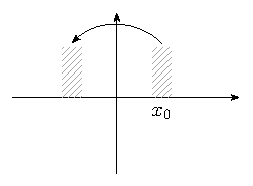
\includegraphics[scale=0.55]{ch02_fig_2_2_1}
\end{center}

\begin{corollary}[(Convergence rate)]
Under the same conditions,
\[
|y_n(x) - y(x)| \le \frac{ML^n}{(n+1)!}\,|x - x_0|^{n+1}, \qquad \forall\, x \in [x_0 - h,\ x_0 + h].
\]
\end{corollary}

\begin{example}
$\frac{dy}{dx} = x^2 + y^2$: for any $(x_0, y_0)$ there is a unique solution curve through it
(because $f(x,y) = x^2 + y^2$ is Lipschitz on every bounded domain).
\end{example}

\begin{example}
$\frac{dy}{dx} = y^{1/3}$: for $(x_0, y_0)$ there is a unique solution curve through it if
$y_0 \neq 0$ (because $f(x,y) = y^{1/3}$ is Lipschitz on domains where $y \neq 0$).
\end{example}

\begin{remark}
Picard--Lindel\"of holds for $y(x): I \subseteq \R \to X$ with $X$ a complete metric space.
\end{remark}

\begin{example}[(Miller, 1923)]
$y' = f(x,y)$, $y(0) = 0$, where
\[
f(x,y) = \begin{cases} 0 & ,\ x = 0,\ y \in \R \\ 2x & ,\ 0 \le x \le 1,\ y \le 0 \\
2x - \dfrac{4y}{x} & ,\ 0 < x \le 1,\ 0 < y < x^2 \\ -2x & ,\ 0 < x \le 1,\ y \ge x^2 \end{cases}
\]
\begin{center}
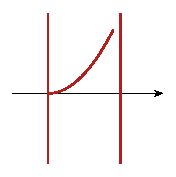
\includegraphics[scale=0.5]{ch02_fig_2_3_1}
\end{center}
$f(x,y)$ is continuous but not Lipschitz (notice $\frac{4|y_1 - y_2|}{|x|}$ near $x = 0$).

Picard sequence: $y_0(x) \equiv 0$, $y_1(x) = x^2$, $y_2(x) = -x^2$, $y_3(x) = x^2$, \ldots

But $f(x,y)$ is decreasing in $y$.
\end{example}

\secn{2.3\quad Peano's thm \& Osgood uniqueness}

\begin{theorem}[(Peano)]
For $\begin{cases} y' = f(x,y) \\ y(x_0) = y_0 \end{cases}$ with
$D := \{(x,y) :\ |x - x_0| \le a,\ |y - y_0| \le b\}$ and $f \in C(D)$,
the Cauchy problem has \textbf{at least one solution} on
$x \in [x_0 - h,\ x_0 + h]$, $h := \min\{a,\ b/M\}$, $M := \max_D f(x,y)$.
\end{theorem}

\textbf{Pf.} For simplicity, construct the solution on $[x_0, x_0 + h]$ only. For each $n$, cut
$[x_0, x_0 + h]$ into $n$ segments, $x_k := x_0 + \frac{k}{n} h$. Construct, for
$x \in [x_k, x_{k+1}]$,
\[
y_n(x) = y_0 + \sum_{j=0}^{k-1} f(x_j, y_j)(x_{j+1} - x_j) + f(x_k, y_k)(x - x_k),
\qquad y_j := y_n(x_j).
\]
\begin{center}
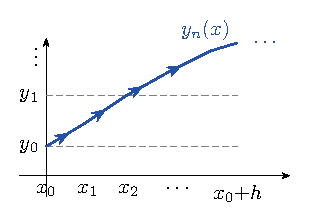
\includegraphics[scale=0.55]{ch02_fig_2_3_2}
\end{center}

Properties of $y_n$:
\begin{itemize}
\item[(1)] $y_n \in C[x_0, x_0 + h]$ for all $n$.
\item[(2)] $|y_n(x) - y_0| \le Mh$ for all $n$ (uniformly bounded).
\item[(3)] $|y_n(x) - y_n(\tilde{x})| \le M$ for all $n$ and $x, \tilde{x} \in [x_0, x_0 + h]$
(taking $x$ as a starting point, $y_n(\tilde{x})$ varies by at most $M$).
\begin{center}
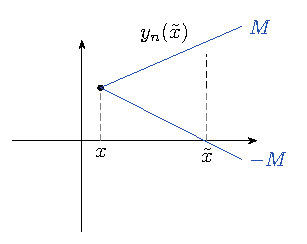
\includegraphics[scale=0.5]{ch02_fig_2_3_3}
\end{center}
\item[(4)] $y_n(x)$ approximates the solution:
\[
\Bigl|\, y_n(x) - \Bigl[\, y_0 + \int_{x_0}^{x} f(s, y_n(s))\, ds \,\Bigr]\Bigr|
\le \sum_{j=0}^{k-1} \int_{x_j}^{x_{j+1}} |f(x_j, y_j) - f(s, y_n(s))|\, ds
+ \int_{x_k}^{x} |f(x_k, y_k) - f(s, y_n(s))|\, ds < \varepsilon h
\]
(taking $n \to \infty$, using $f \in C(D) \Rightarrow$ uniformly continuous). By the A--A lemma we
find $y_{n_k}(x) \Rightarrow y(x)$ on $[x_0, x_0 + h]$; easily
$\bigl|y(x) - [y_0 + \int_{x_0}^{x} f(s, y(s))\,ds]\bigr| < \varepsilon(1 + 2h)$.
Hence $y(x)$ solves the equation. \qed
\end{itemize}

\begin{definition}
$f(x,y) \in C(\Omega)$ \& $|f(x,y_1) - f(x,y_2)| < F(|y_1 - y_2|)$, where
$F \in C(0, +\infty)$ \& $\int_0^{\varepsilon} \frac{dr}{F(r)} = +\infty$ for all $\varepsilon > 0$.
Then $f(x,y)$ satisfies the \textbf{Osgood condition} on $\Omega$ w.r.t.\ $y$.
\end{definition}

\begin{theorem}[(Osgood)]
For the equation in Peano's thm., if $f(x,y)$ satisfies the Osgood condition, then the solution is unique.
\end{theorem}

\textbf{Pf.} Suppose $\varphi_1(x), \varphi_2(x)$ are two different solutions with
$\varphi_1(x_0) = \varphi_2(x_0)$; $\exists\, x_1$: $\varphi_1(x_1) \neq \varphi_2(x_1)$.
Assume $x_1 > x_0$ \& $\varphi_1(x_1) > \varphi_2(x_1)$ and set
\[
r(x) := \varphi_1(x) - \varphi_2(x), \qquad x^* := \sup\{x \in [x_0, x_1] : r(x) = 0\},
\]
so $r(x^*) = 0$ and $r(x) > 0$ for $x \in (x^*, x_1]$. Then
\[
r'(x) = f(x, \varphi_1(x)) - f(x, \varphi_2(x)) \le F(|\varphi_1(x) - \varphi_2(x)|) = F(r(x)),
\qquad x \in (x^*, x_1],
\]
\[
\Rightarrow\ \frac{r'(x)}{F(r(x))} \le 1
\ \Rightarrow\ \int_{x^*}^{x_1} \frac{r'(x)}{F(r(x))}\, dx \le x_1 - x^*
\ \Rightarrow\ +\infty \le x_1 - x^*,
\]
a contradiction. \qed

\begin{proposition}
For the equation in Peano's thm., if $f(x,y)$ is decreasing w.r.t.\ $y$, then the solution is unique.

\textbf{Pf.} With $\varphi_1, \varphi_2, r(x), x^*$ as above:
$r'(x) = f(x, \varphi_1) - f(x, \varphi_2) \le 0$ on $[x^*, x_1]$, so $r(x) \downarrow$;
but $r(x^*) = 0$ and $r(x_1) > 0$. \qed
\end{proposition}

\begin{exercise}
$y' = \begin{cases} 0 & ,\ y = 0 \\ y \ln|y| & ,\ y \neq 0 \end{cases}$:
the solution exists \& is unique.

\textbf{Pf.} For $(x_0, y_0) \in \R^2$: if $y_0 \neq 0$, use Picard--Lindel\"of; if $y_0 = 0$,
existence holds by Peano's thm. Notice $y \equiv 0$ is a solution; if $\varphi(x)$ were another
solution, then on $(x^*, x_1]$
\[
\int_{x^*}^{x_1} \frac{\varphi'(x)}{\varphi(x) \ln|\varphi(x)|}\, dx
= \ln\bigl|\ln|\varphi(x)|\bigr|\Big|_{\varphi(x^*)}^{\varphi(x_1)} = +\infty,
\]
so the assumption is wrong. \qed
\end{exercise}

\secn{2.4\quad Extension of solutions}

\begin{theorem}[(Extension of solutions)]
For $\begin{cases} y' = f(x,y) \\ y(x_0) = y_0 \end{cases}$ with $f \in C(\Omega)$, $\Omega$ a
domain in $\R \times \R^n$: any solution curve $\Gamma$ must extend to the boundary of $\Omega$,
i.e.\ for every compact $\Omega_1 \ni (x_0, y_0)$, $\Gamma$ extends into $\Omega \setminus \Omega_1$.
\end{theorem}

\begin{center}
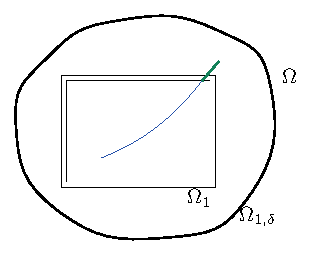
\includegraphics[scale=0.55]{ch02_fig_2_4_1}
\end{center}

\begin{definition}
$y_1$ \& $y_2$ are two solutions of $\begin{cases} y' = f(x,y) \\ y_0 = y(x_0) \end{cases}$:
if $\mathrm{domain}(y_2) \supseteq \mathrm{domain}(y_1)$ and $y_2 = y_1$ on the common domain, we
say $y_2$ is an \textbf{extension} of $y_1$.
\end{definition}

\begin{definition}
$y(x)$ is called a \textbf{maximal solution} if it is defined on an open interval and cannot be
extended. Denote $(T_-, T_+) := \mathrm{domain}(y)$.
\end{definition}

\begin{theorem}
Suppose $\Omega$ is a domain and $f \in C(\Omega)$. For every $(x_0, y_0)$ there \textbf{exists a
maximal solution} of the Cauchy problem.
\end{theorem}

\textbf{Pf.} We prove it for the easier case (assuming local uniqueness). Let
$S = \{$ all solutions on an open interval $\}$. For $\varphi \in S$ let $I_\varphi$ be its open
interval; denote $I = \bigcup_{\varphi \in S} I_\varphi$, clearly open. We show $I$ is an interval:
$a := \inf\{x \in I\}$, $b := \sup\{x \in I\}$; for $x^* \in (a,b)$, choose $x_1 \in I$ with
$x^* < x_1 < b$ close to $x^*$; take $\varphi \in S$ with $x_1 \in I_\varphi$; since $I_\varphi$ is
an open interval, $x^* \in I_\varphi \Rightarrow x^* \in I$. Thus $I = (a,b)$. Define $y_m = \varphi$
on each $I_\varphi$ (unique by assumption; otherwise use Zorn's lemma). It is easy to check that
$y_m$ is a maximal solution. \qed

\begin{corollary}
If $I_{\max} = (T_-, T_+)$ with $T_+ < +\infty$, then for every compact $CC$ with
$[x_0, T_+] \times C \subseteq \Omega$, the solution must leave $[x_0, T_+] \times C$.
($y$ bounded $\Rightarrow x$ extended.)
\end{corollary}

\begin{exercise}
$y' = (x^2 + y^2 + 1)\sin \pi y$: any solution exists on $\R$ and is monotonic.

\textbf{Pf.} $f(x,y) \in C^1(\R^2)$, hence locally Lipschitz. Notice $y = n \in \Z \Rightarrow y' = 0$,
so $y \equiv n$ are solutions.
\begin{center}
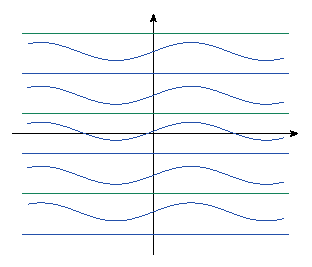
\includegraphics[scale=0.55]{ch02_fig_2_4_2}
\end{center}
For $y_0 = n$: the unique solution is $y \equiv n$, global. For $n < y_0 < n+1$: the unique solution
cannot cross $y = n$ \& $y = n+1$, hence is global. The sign of $y'$ depends only on $y$, so $y$ is
monotonic. \qed
\end{exercise}

\begin{exercise}
$y' = (y^2 - 2y - 3)\,e^{(x+y)^2}$: any solution with $I_{\max} = (T_-, T_+)$ has
$T_- = -\infty$ or $T_+ = +\infty$.

\textbf{Pf.} $f(x,y) \in C^1(\R)$, hence locally Lipschitz. Also $y \equiv 3$ \& $y \equiv -1$ are
global solutions.
\begin{center}
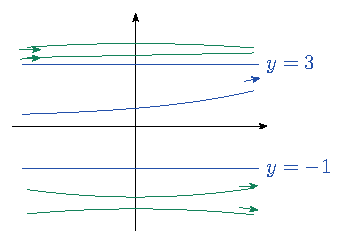
\includegraphics[scale=0.55]{ch02_fig_2_4_3}
\end{center}
For $y_0 > 3$: the solution cannot cross $y = 3$ and is increasing, so $T_- = -\infty$.
For $y_0 < -1$: the solution cannot cross $y = -1$ and is increasing, so $T_+ = +\infty$. \qed
\end{exercise}

\begin{exercise}[(Liouville)]
$y' = x^2 + y^2$: any solution must have a bounded lifespan.

\textbf{Pf.} WLOG $x_0 \ge 0$; look at the solution $\varphi$ on $(T_-, T_+)$ and show $T_+ < +\infty$
(same for $T_-$). Fix $x_1 \in (x_0, T_+)$: $\varphi'(x) = x^2 + \varphi^2(x) \ge x_1^2 + \varphi^2(x)$
for $x > x_1$, so
\[
\frac{\varphi'(x)}{x_1^2 + \varphi^2(x)} \ge 1
\ \Rightarrow\ \int_{x_1}^{z} \frac{\varphi'(x)}{x_1^2 + \varphi^2(x)}\, dx \ge z - x_1
\ \Rightarrow\ \frac{\pi}{x_1} \ge z - x_1
\ \Rightarrow\ z \le x_1 + \frac{\pi}{x_1}
\]
(in fact we use the comparison lemma). Letting $z \to T_+$ gives $T_+ < +\infty$. \qed
\end{exercise}

\begin{exercise}
$\begin{cases} y' = f(x,y) \\ y_0 = y(x_0) \end{cases}$ with $f \in C(\R^2)$ satisfying
\[
|f(x,y)| \le M(T) + L(T)\,|y|, \qquad \forall\, T,\ \forall\, (x,y) \in [-T, T] \times \R,
\]
where $M, L > 0$ are continuous functions. Then any solution is global.

\textbf{Pf.} For $[x_0, T]$ with $T$ large enough:
\[
|y(x)| \le |y_0| + \int_{x_0}^{x} \bigl(M(T) + L(T)\,|y(s)|\bigr)\, ds
\le \bigl(|y_0| + M(T)(T - x_0)\bigr)\, e^{L(T)(x - x_0)} \quad \text{(Gronwall)}.
\]
Hence $|y(x)|$ is bounded on $[x_0, T]$ and the solution extends to $+\infty$; similarly for the
negative direction. \qed
\end{exercise}

\secn{2.5\quad Comparison lemma}

\begin{lemma}[(1st comparison principle)]
$\Omega$ is a domain, $f, F \in C(\Omega)$ \& $F > f$ on $\Omega$ (strictly). If
$\begin{cases} y' = f(x,y) \\ y(x_0) = y_0 \end{cases}$ has solution $\varphi$ and
$\begin{cases} y' = F(x,y) \\ y(x_0) = y_0 \end{cases}$ has solution $\psi$ on $(a,b) \ni x_0$, then
$\varphi(x) > \psi(x)$ for $x \in (a, x_0)$ and $\varphi(x) < \psi(x)$ for $x \in (x_0, b)$.
\end{lemma}

\textbf{Pf.} $h(x) := \psi(x) - \varphi(x)$, $h(x_0) = 0$, $h'(x) > 0$ on $(a,b)$; then
$\exists\,\delta$ s.t.\ $h(x) > 0$ on $(x_0, x_0 + \delta)$, $h(x) < 0$ on $(x_0 - \delta, x_0)$
(using here). Suppose $h(x) > 0$ fails on $(x_0, b)$; then $\exists\, x_1$ s.t.\ $h(x_1) \le 0$.
Take
\[
x^* = \inf\{x \in (x_0, b) : h(x) \le 0\};
\]
then $h(x^*) = 0$ \& $h'(x^*) < 0$, a contradiction. Similarly for the other side. \qed

\begin{exercise}
$y' = f(x,y)$ with $f \in C(\Omega)$ \& $|f| \le A(x)|y| + B(x)$ on $\Omega = (a,b) \times \R$,
where $A(x), B(x) > 0$ are continuous on $(a,b)$. Then any solution has lifespan $I_{\max} = (a,b)$.
(We don't know whether the solution is unique, so we construct objects to compare.)

\textbf{Pf.} Let $F := A(x)|y| + B(x) + 1$ and $G := -F$. The equation with $F$ has a unique
solution ($F$ locally Lipschitz), which is strictly increasing, thus has at most one zero on
$I_{\max}$. Case 1: no zero; WLOG $y(x) > 0$, then $y' = A(x)y + B(x)$, $y(x_0) = y_0$ is a first
order ODE with a solution on $(a,b)$. Case 2: one zero $x_1$; derive two equations
\[
\begin{cases} y' = A(x)y + B(x) \\ y(x_1) = 0 \end{cases} \text{ on } x > x_1,
\qquad \begin{cases} y' = -A(x)y + B(x) \\ y(x_1) = 0 \end{cases} \text{ on } x < x_1,
\]
each with a solution on $(a,b)$. Same for $G$. By the 1st comparison lemma the solution of the
original equation is bounded on every compact $C \subseteq (a,b)$, thus global. \qed
\end{exercise}

\begin{definition}
Consider $y' = f(x,y)$ with $f \in C(\Omega)$; a solution exists by Peano's thm. If $y_1, y_2$ are
two solutions on an interval $I$ satisfying $\forall$ solutions $y(x)$ on $I$:
$y_1(x) \le y(x) \le y_2(x)$, we call $y_2(x)$ a \textbf{sup-solution} and $y_1(x)$ a
\textbf{sub-solution}.
\end{definition}

\begin{center}
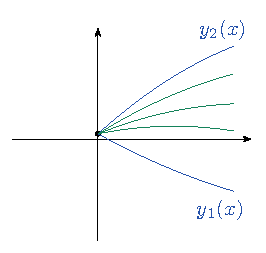
\includegraphics[scale=0.5]{ch02_fig_2_5_1}
\end{center}

\begin{theorem}
$f(x,y) \in C(D)$; then $\exists\, \tau > 0$ s.t.\ a sup-solution and a sub-solution exist on
$\{x : |x - x_0| < \tau\}$.
\end{theorem}

\textbf{Pf.} (Create $f_n$ to use the comparison principle.) Set
$f_n(x,y) = f(x,y) + \varepsilon_n$, $\varepsilon_n \downarrow 0+$. By Peano's thm the problem
$y' = f_n(x,y)$, $y(x_0) = y_0$ has a solution $\varphi_n(x)$ on $[x_0 - h_n, x_0 + h_n]$ with
\[
h_n := \min\Bigl\{a,\ \frac{b}{M_n}\Bigr\}, \qquad M_n := \sup_D |f_n(x,y)|.
\]
$|\varphi_n(x) - y_0| \le b$ for all $n$ (uniformly bounded), and
\[
|\varphi_n(x) - \varphi_n(x')| = \Bigl|\int_x^{x'} f_n(s, y_n(s))\, ds\Bigr| \le M_n|x - x'| \le (M+1)|x - x'|
\]
(equicontinuous). Take $\tau < h$; then $\{|x - x_0| < \tau\} \subseteq \{|x - x_0| \le h_n\}$ for
$n$ large. Apply A--A on $[x_0 - \tau, x_0 + \tau]$: $\exists\ \varphi_{n_k} \Rightarrow \varphi$,
where $\varphi$ solves the original IVP. Since $f_n = f + \varepsilon_n \to f$, we get
$\varphi_n(x) > \varphi(x)$ for $x > x_0$ and $\varphi_n(x) < \varphi(x)$ for $x < x_0$.
Taking the $h_k$ limit: $\varphi$ is a sup-solution on $(x_0, x_0 + \tau)$ and a sub-solution on
$(x_0 - \tau, x_0)$. Redo with $\varepsilon_n \uparrow 0-$ for the other side. \qed

\begin{theorem}[(2nd comparison)]
Consider
\[
\begin{cases} y' = f(x,y) \\ y(x_0) = y_0 \end{cases}\ (\times)
\qquad \begin{cases} y' = F(x,y) \\ y(x_0) = y_0 \end{cases}\ (\times\times)
\qquad f(x,y) \le F(x,y) \ \text{(not strictly)}.
\]
Let $\varphi(x)$ be a sub-solution on $[x_0, b)$ \& sup-solution on $(a, x_0]$ for $(\times)$; let
$\psi(x)$ be a sup-solution on $[x_0, b)$ \& sub-solution on $(a, x_0]$ for $(\times\times)$. Then
$\varphi(x) \le \psi(x)$ for $x \ge x_0$ and $\varphi(x) \ge \psi(x)$ for $x \le x_0$.
\end{theorem}

\textbf{Pf.} Solve $y' = F(x,y) + \varepsilon_n$, $y(x_0) = y_0$ ($\varepsilon_n \downarrow 0$) to get
$\psi_n(x)$; solve $y' = f(x,y) - \varepsilon_n$ to get $\varphi_n(x)$ (we have to construct a strict
inequality). From the existence of sup \& sub solutions, $\psi_{n,k} \Rightarrow \psi$ and
$\varphi_{n,k} \Rightarrow \varphi$. By the 1st comparison lemma we obtain the claim. \qed

\begin{exercise}[starred]
$y' = x^2 + (y+1)^2$, $y(0) = 0$: the lifespan $(T_-, T_+)$ satisfies $T_+ \in (\pi/4,\, 1)$.

\textbf{Pf.} The solution is unique and has bounded lifespan.
\textbf{Step 1.} $T_+ \in [\pi/4, 1]$: consider $|x| \le 1$ and compare with
$y' = (y+1)^2$ and $y' = 1 + (y+1)^2$, $y(0)=0$:
\[
\frac{-1}{x-1} - 1 \le y(x) \le \tan\Bigl(x + \frac{\pi}{4}\Bigr) - 1
\qquad \text{on } [0,1],
\]
where $\frac{-1}{x-1} - 1$ exists on $[0,1)$ and $\tan(x+\frac{\pi}{4}) - 1$ exists on $[0, \frac{\pi}{4})$.
Hence $T_+ \in [\pi/4, 1]$.
\textbf{Step 2.} $T_+ \in (\pi/4, 1)$: notice $y' > 0$, so $x = \varphi(y)$ with
$\varphi'(y) = \frac{1}{x^2 + (y+1)^2}$ and $\lim_{y\to+\infty}\varphi(y) = T_+$; thus
\[
T_+ = \int_0^{+\infty} \frac{ds}{x^2 + (s+1)^2},
\qquad
\int_0^{+\infty} \frac{ds}{1 + (s+1)^2} < T_+ < \int_0^{+\infty} \frac{ds}{(s+1)^2},
\]
using $0 \le x < T_+ \le 1$. Hence $\frac{\pi}{4} < T_+ < 1$. \qed
\end{exercise}

\secn{2.6\quad Dependence on data \& parameter}

\begin{question}
Does a small perturbation of the data / parameter yield a small / big difference of the solution?
\end{question}

We can always combine the two problems. Original problem:
$\begin{cases} y' = f(x,y,\lambda) \\ y(x_0) = y_0 \end{cases}$.

\textbf{Reduction \#1.} $u := y - y_0$, $t := x - x_0$:
\[
\begin{cases} u'(t) = g(u, t, \Lambda) \\ u(0) = 0 \end{cases},
\qquad \Lambda := (x_0, y_0, \lambda).
\]

\textbf{Reduction \#2.} Consider $U(x) = (y(x)\ \ z(x))^T$ with
$\begin{cases} y' = f(x,y,\lambda) \\ y(x_0) = y_0 \end{cases}$ and
$\begin{cases} z' = 0 \\ z(x_0) = \lambda \end{cases}$; then
$U'(x) = F(x, U) = \begin{pmatrix} f(x,y,z) \\ 0 \end{pmatrix}$, $U(x_0) = \begin{pmatrix} y_0 \\ \lambda \end{pmatrix}$.

So we should discuss equations with $y \in \R^n$:
$y : \R \to \R^n$, $f : \R \times \R^n \to \R^n$, $\begin{cases} y' = f(x,y) \\ y(x_0) = y_0 \end{cases}$,
satisfying (1) Picard--Lindel\"of, (2) Peano, (3) Extension --- all proved. And:

(4) $y' = A(x)y + b(x)$ with $A(x), b(x) \in C(a,b)$: the solution is unique and extends to $(a,b)$.

\textbf{Pf.} It suffices to show $y(x)$ is bounded on $(c,d) \subseteq (a,b)$:
\[
\frac{d}{dx}\| y(x) \|^2 = y(x)^T \bigl( A(x)y + b(x) \bigr) + \bigl( y^T A^T + b^T \bigr) y(x)
\le 2\, \| y(x) \|\,\bigl( \| A(x) \|\,\| y(x) \| + \| b(x) \| \bigr),
\]
\[
\Rightarrow\ \frac{d}{dx}\| y(x) \| \le \| A(x) \|\,\| y(x) \| + \| b(x) \| \le M \| y(x) \| + N.
\]
By Gronwall, $\|y(x)\|$ is bounded. \qed

\subsecn{2.6.1\quad Continuous dependence}

\begin{theorem}[(Continuous dependence)]
$\Omega$ a bounded region of $\R \times \R^n$,
$\begin{cases} y' = f(x,y) \\ y(x_0) = y_0 \end{cases}$ with $f \in C(\Omega)$; assume the solution
is unique on a closed interval $I_0$ for every $(x_0, y_0)$. Then the solution
$\varphi(x\,;\, x_0, y_0)$ is continuous w.r.t.\ $(x_0, y_0)$: $\forall \varepsilon > 0\ \exists \delta > 0$ s.t.\
$\| x_0 - \tilde{x}_0 \| + \| y_0 - \tilde{y}_0 \| < \delta$ implies
\[
\| \varphi(x\,;\, x_0, y_0) - \varphi(x\,;\, \tilde{x}_0, \tilde{y}_0) \| < \varepsilon,
\qquad \forall x \in I_0.
\]
\end{theorem}

\textbf{Pf.} Suppose not: $\exists \varepsilon_0 > 0$ and, for all $n$, points with
$\| (x_0^{(n)}, y_0^{(n)}) - (x_0, y_0) \| < \frac{1}{n}$ and
$\| \varphi(x_n; x_0^{(n)}, y_0^{(n)}) - \varphi(x_n; x_0, y_0) \| \ge \varepsilon_0$.
Since $I_0$ is compact, $\exists \{ x_{n_k} \} \subseteq \{ x_n \}$: $x_{n_k} \Rightarrow x^* \in I_0$.

Check: $\varphi(x\,;\, x_0^{(n)}, y_0^{(n)})$ is uniformly bounded \& equicontinuous:
(1) $\varphi = y_0^{(n)} + \int_{x_0^{(n)}}^x f(s, \varphi(s))\, ds$ is uniformly bounded;
(2) $| \varphi(x) - \varphi(\tilde{x}) | = \bigl|\int_x^{\tilde{x}} f(s, \varphi(s))\, ds\bigr| \le M|x - \tilde{x}|$.

By the A--A lemma, $\varphi(x\,;\, x_0^{(n_k)}, y_0^{(n_k)}) \Rightarrow \widetilde{\varphi}(x)$.
The IVP has a unique solution, so $\widetilde{\varphi}(x) = \varphi(x\,;\, x_0, y_0)$. Taking the
limit in $x$:
\[
0 = \bigl\| \varphi(x^*\,;\, x_0, y_0) - \varphi(x^*\,;\, x_0, y_0) \bigr\| \ge \varepsilon_0,
\]
a contradiction. \qed

\begin{lemma}[(Quantitative bound)]
For $\begin{cases} y' = f(x,y) \\ y(x_0) = y_0 \end{cases}$ and
$\begin{cases} y' = f(x,y) \\ y(x_0) = \tilde{y}_0 \end{cases}$ with corresponding $\varphi, \psi$ on $I$:
\[
| \varphi(x) - \psi(x) | \le | y_0 - \tilde{y}_0 |\, e^{L|x - x_0|},
\]
where $L$ is a Lipschitz constant of $f$.

\textbf{Pf.} WLOG $x_0 = 0$:
$| \varphi - \psi | = \bigl| y_0 - \tilde{y}_0 + \int_{x_0}^x f(s, \varphi(s)) - f(s, \psi(s))\, ds \bigr|$;
apply Gronwall. \qed
\end{lemma}

\subsecn{2.6.2\quad $C^1$ dependence on data \& parameters}

\begin{theorem}[($C^1$ dependence)]
$\begin{cases} y' = f(x,y,\lambda) \\ y(0) = 0 \end{cases}$ with
$\Omega = \{ \|x\| \le a,\ \|y\| \le b,\ \|\lambda\| \le c \}$, $f \in C(\Omega)$,
$f_y, f_\lambda \in C(\Omega)$. Then the solution $y = \varphi(x, \lambda) \in C^1(D)$, where
\[
D := \{ |x| \le h,\ |\lambda| < c \}, \qquad h := \min \Bigl\{ a,\ \frac{b}{M_f} \Bigr\}.
\]
\end{theorem}

\textbf{Pf.} $\varphi(x, \lambda)$ is $C^1$ in $x$; we only need $\lambda$.
$\varphi(x, \lambda) = \int_0^x f(s, \varphi(s, \lambda), \lambda)\, ds$. If $\varphi$ were
differentiable in $\lambda$, then $u := \frac{\partial \varphi}{\partial \lambda}$ would satisfy
the first order ODE
\begin{equation}
\begin{cases} \dfrac{du}{dx} = \dfrac{\partial f}{\partial y}(x, \varphi(x,\lambda), \lambda)\, u
+ \dfrac{\partial f}{\partial \lambda}(x, \varphi(x,\lambda), \lambda) \\ u(0, \lambda) = 0 \end{cases}
\quad (\times)
\end{equation}
So we only have to prove: \textcircled{1} $(\times)$ has a unique solution on $|x| \le h$, $|\lambda| \le C$
(first order ODE theory); \textcircled{2} the solution of $(\times)$ is the derivative, i.e.
\[
| \varphi(x, \lambda) - \varphi(x, \lambda_0) - u(x, \lambda_0)(\lambda - \lambda_0) | = o(|\lambda - \lambda_0|).
\]
For \textcircled{2}, expand:
\begin{align*}
&\ \varphi(x, \lambda) - \varphi(x, \lambda_0) - u(x, \lambda_0)(\lambda - \lambda_0)\\
&= \int_0^x f(s, \varphi(s, \lambda), \lambda)\, ds - \int_0^x f(s, \varphi(s, \lambda_0), \lambda_0)\, ds\\
&\quad - \int_0^x \Bigl[ \frac{\partial f}{\partial y}(s, \varphi(s, \lambda_0), \lambda_0)\, u(s, \lambda_0)
+ \frac{\partial f}{\partial \lambda}(s, \varphi(s, \lambda_0), \lambda_0) \Bigr] (\lambda - \lambda_0)\, ds\\
&= \int_0^x \!\!\int_0^1 \frac{\partial f}{\partial \lambda}\bigl(s, \varphi(s, \lambda),\, \theta\lambda + (1-\theta)\lambda_0\bigr) d\theta\,(\lambda - \lambda_0)\, ds
+ \int_0^x \!\!\int_0^1 \frac{\partial f}{\partial y}\bigl(s,\, \theta\varphi(s, \lambda) + (1-\theta)\varphi(s, \lambda_0),\, \lambda_0\bigr) d\theta\,\bigl(\varphi(s, \lambda) - \varphi(s, \lambda_0)\bigr) ds\\
&\quad - \int_0^x \frac{\partial f}{\partial y}(s, \varphi(s, \lambda_0), \lambda_0)\, u(s, \lambda_0)\, (\lambda - \lambda_0)\, ds
- \int_0^x \frac{\partial f}{\partial \lambda}(s, \varphi(s, \lambda_0), \lambda_0)\, (\lambda - \lambda_0)\, ds\\
&= \int_0^x \!\!\int_0^1 \Bigl[ \frac{\partial f}{\partial \lambda}\bigl(s, \varphi(s, \lambda), \theta\lambda + (1-\theta)\lambda_0\bigr) - \frac{\partial f}{\partial \lambda}(s, \varphi(s, \lambda_0), \lambda_0) \Bigr] d\theta\, ds\,(\lambda - \lambda_0)\\
&\quad + \int_0^x \!\!\int_0^1 \frac{\partial f}{\partial y}\bigl(s, \theta\varphi(s, \lambda) + (1-\theta)\varphi(s, \lambda_0), \lambda_0\bigr) d\theta\,
\bigl[ \varphi(s, \lambda) - \varphi(s, \lambda_0) - u(s, \lambda_0)(\lambda - \lambda_0) \bigr] ds\\
&\quad + \int_0^x \!\!\int_0^1 \Bigl[ \frac{\partial f}{\partial y}\bigl(s, \theta\varphi(s, \lambda) + (1-\theta)\varphi(s, \lambda_0), \lambda_0\bigr) - \frac{\partial f}{\partial y}(s, \varphi(s, \lambda_0), \lambda_0) \Bigr] d\theta\, u(s, \lambda_0)(\lambda - \lambda_0)\, ds.
\end{align*}
Denote $\Delta(x) = | \varphi(x, \lambda) - \varphi(x, \lambda_0) - u(x, \lambda_0)(\lambda - \lambda_0) |$.
By continuity of $\frac{\partial f}{\partial y}$, $\frac{\partial f}{\partial \lambda}$ and
$\varphi(x, \lambda)$:
\[
\Delta(x) \le \Bigl| \int_0^x \!\!\int_0^1 \varepsilon_1\, d\theta\, ds\,(\lambda - \lambda_0) \Bigr|
+ \Bigl| \int_0^x \!\!\int_0^1 K\, d\theta\, \Delta(s)\, ds \Bigr|
+ \Bigl| \int_0^x \!\!\int_0^1 \varepsilon_1\, d\theta\, K(\lambda - \lambda_0)\, ds \Bigr|.
\]
For $x \in [0, h]$: $\Delta(x) \le \varepsilon_1 h |\lambda - \lambda_0| + \varepsilon_1 K h |\lambda - \lambda_0| + K\int_0^x \Delta(s)\, ds$.
By Gronwall, $\Delta(x) \le \varepsilon_1 (K+1) h\, |\lambda - \lambda_0|\, e^{Kx}$, hence
\[
\frac{\Delta(x)}{|\lambda - \lambda_0|} \le \varepsilon_1 (K+1) h\, e^{Kh} < \varepsilon
\quad \Rightarrow \quad \lim_{\lambda \to \lambda_0} \frac{\Delta(x)}{|\lambda - \lambda_0|} = 0.
\]
Similar proof for $x \in [-h, 0]$. \qed

\begin{corollary}
If $f \in C^k(\Omega)$, then the solution $\varphi(x, \lambda)$ is $C^k$ on $D$ (by induction).
\end{corollary}

\begin{theorem}
If $f$ is analytic in $\Omega$ (or analytic w.r.t.\ $\lambda$), then the solution is analytic in $D$
(or analytic w.r.t.\ $\lambda$).
\end{theorem}

\begin{example}
$\begin{cases} \frac{dy}{dx} = y + \lambda(x + y^2) \\ y(0) = 1 \end{cases}$: find
$\frac{\partial y}{\partial \lambda}\big|_{\lambda = 0}$.

\textbf{Sol.} $y(x, \lambda) = 1 + \int_0^x y(s, \lambda) + \lambda(s + y^2(s, \lambda))\, ds$, so
\[
\frac{\partial y}{\partial \lambda}(x, \lambda) = \int_0^x \frac{\partial y}{\partial \lambda}(s, \lambda) + s + y^2(s, \lambda) + 2\lambda\, y(s, \lambda)\, \frac{\partial y}{\partial \lambda}(s, \lambda)\, ds;
\]
hence $u(x, \lambda) := \frac{\partial y}{\partial \lambda}(x, \lambda)$ solves
\[
\begin{cases} \frac{d}{dx} u(x, \lambda) = (1 + 2\lambda\, y(x, \lambda))\, u(x, \lambda) + (x + y^2(x, \lambda)) \\ u(0, \lambda) = 0. \end{cases}
\]
Solving the first order ODE:
$e^{-\int_0^x A(s)\, ds}\, u(x, \lambda) = \int_0^x e^{-\int_0^z A(s)\, ds}\, B(z)\, dz$ with
$A = 1 + 2\lambda y$, $B = x + y^2$. Plug in $\lambda = 0$:
\[
e^{-x}\, u(x, 0) = \int_0^x (z e^{-z} + e^z)\, dz = e^x - e^{-x}(x+1),
\qquad\text{hence}\quad u(x, 0) = e^{2x} - (x+1). \quad\qed
\]
\end{example}

%======================================================================
\chap{Chapter 3\quad Linear Systems}

$y(x) : I \subseteq \R \to \R^n$, $\dfrac{dy}{dx} = A(x)y + f(x)$, $A, f \in C(a,b)$.

\secn{3.1\quad General theory}

\begin{lemma}
The solution of the IVP is \textbf{unique \& extends} to $(a,b)$.

\textbf{Pf.} It suffices to prove $y(x)$ bounded on $(c,d) \subseteq (a,b)$:
\[
\frac{d}{dx}\| y(x) \|^2 = y(x)^T \bigl( A(x)y + f(x) \bigr) + \bigl( y^T A^T + f^T \bigr) y(x)
\le 2\, \| y(x) \|\,\bigl( \| A(x) \|\,\| y(x) \| + \| f(x) \| \bigr),
\]
\[
\Rightarrow\ \frac{d}{dx}\| y(x) \| \le \| A(x) \|\,\| y(x) \| + \| f(x) \| \le M \| y(x) \| + N.
\]
By Gronwall, $\|y(x)\|$ is bounded. \qed
\end{lemma}

\subsecn{3.1.1\quad Homogeneous equation}

\begin{lemma}
$S = \bigl\{ y(x) \text{ solves } \frac{dy}{dx} = A(x)y \bigr\}$ is an $n$-dim vector space.

\textbf{Pf.} Obviously $S$ is a vector space; check the dimension. Consider
$T : \R^n \to S$, $y_0 \mapsto$ the solution $y(x)$ with $y(0) = y_0$. $T$ is linear and bijective,
making $S \cong \R^n$. So $\dim S = n$. \qed
\end{lemma}

\begin{lemma}
There are $n$ linearly independent solutions $\{ y_i(x) \}$ s.t.\ every $f \in S$ is
$y = \sum_{i=1}^n a_i y_i$. We call $\{ y_i(x) \}$ a fundamental system of solutions.

\textbf{Pf.} Using $T$, choose $y_0^{(1)}, \dots, y_0^{(n)}$ to get $y_i(x)$. \qed
\end{lemma}

\begin{definition}
For $n$ solutions of the homogeneous equation, $W(y_1, \dots, y_n) := \det(y_1(x)\ \cdots\ y_n(x))$
is the \textbf{Wronskian determinant}.
\end{definition}

\begin{lemma}[(Liouville identity)]
\[
W(x) = W(x_0)\, e^{\int_{x_0}^x \tr A(s)\, ds}, \qquad \forall\ x_0, x \in (a,b).
\]
\textbf{Pf.} We prove $W'(x) = \tr A(x)\, W(x)$:
\[
W'(x) = \sum_{i=1}^n \begin{vmatrix} y_{11}(x) & y_{21}(x) & \cdots & y_{n1}(x) \\ \vdots & \vdots & & \vdots \\ y'_{1i}(x) & y'_{2i}(x) & \cdots & y'_{ni}(x) \\ \vdots & \vdots & & \vdots \\ y_{1n}(x) & y_{2n}(x) & \cdots & y_{nn}(x) \end{vmatrix},
\qquad
y_k'(x) = A(x)\, y_k(x) \ \Rightarrow\ y'_{kl} = \sum_{m=1}^n a_{lm}\, y_{km}.
\]
\begin{center}
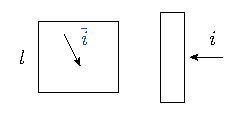
\includegraphics[scale=0.45]{ch03_fig_3_1_1}
\end{center}
Thus
\[
\begin{vmatrix} y_{11}(x) & y_{21}(x) & \cdots & y_{n1}(x) \\ \sum_m a_{im} y_{1m} & \sum_m a_{im} y_{2m} & \cdots & \sum_m a_{im} y_{nm} \\ \vdots & \vdots & & \vdots \\ y_{1n}(x) & y_{2n}(x) & \cdots & y_{nn}(x) \end{vmatrix}
= a_{\bar{i}\bar{i}}\, W(x)
\]
(only if $m = i$ is the determinant nonzero). Hence
$W'(x) = \tr(A(x))\, W(x)$, and $W(x) = W(x_0)\, e^{\int_{x_0}^x \tr A(s)\, ds}$. \qed
\end{lemma}

\begin{lemma}
$y_1(x), \dots, y_n(x) \in S$ are linearly dependent
$\iff W(x) \equiv 0$ on $(a,b) \iff W(x_0) = 0$ for some $x_0 \in (a,b)$.

\textbf{Pf.} The first equivalence is the definition; the second follows from the Liouville identity. \qed
\end{lemma}

\begin{definition}
Suppose $y_1(x), \dots, y_n(x)$ are fundamental solutions of $y' = Ay$; denote
$Y := (y_1\ \ y_2\ \cdots\ y_n)$ a \textbf{fundamental matrix}. If $Y(x_0) = I_n$, we call $Y$ a
principal fundamental matrix.
\end{definition}

\begin{lemma}
(1) If $\Phi(x)$ is a fundamental matrix and $C \in M_n(\R)$ is constant with $\det C \neq 0$, then
$\Phi\, C$ is also a fundamental matrix.

(2) Any two fundamental matrices differ by a constant nonsingular matrix: $\forall\ \Phi, \Psi$,
$\exists\ C$ with $\det C \neq 0$ \& $\Psi = \Phi\, C$.

(3) Given any initial data $y(x_0)$, the solution is $y(x) = \Phi(x)\alpha$ with
$y(x_0) = \Phi(x_0)\alpha$, $\alpha \in \R^n$ constant.

\textbf{Pf.} (1) $(\Phi C)' = \Phi' C = A\Phi C$, $\det(\Phi C) \neq 0$.

(2) Consider $\Phi^{-1}(x)\Psi(x)$:
\[
\frac{d}{dx}\Bigl(\Phi^{-1}(x)\Psi(x)\Bigr)
= \Bigl(-\Phi^{-1}\,\frac{d}{dx}\Phi\,\Phi^{-1}\Bigr)\Psi(x) + \Phi^{-1}\,\frac{d}{dx}\Psi
= \bigl(-\Phi^{-1} A\Phi \Phi^{-1}\bigr)\Psi(x) + \Phi^{-1} A\Psi \equiv 0,
\]
hence $\Phi^{-1}(x)\Psi(x) = C$ with $\det C \neq 0$.

(3) Take $\alpha \in \R^n$ s.t.\ $y(x_0) = \Phi(x_0)\alpha$; then $\Phi(x)\alpha$ solves the IVP. \qed
\end{lemma}

\subsecn{3.1.2\quad Inhomogeneous equation $y' = A(x)y + f(x)$}

\begin{lemma}
The general solution has the form
$\varphi(x) = \Phi(x)\, C + \varphi^*(x)$,
where $\Phi(x)$ is a fundamental matrix of $y' = A(x)y$ and $\varphi^*(x)$ is any solution of
$y' = A(x)y + f(x)$.
\end{lemma}

\begin{lemma}
The general solution has the form
\[
\varphi(x) = \Phi(x)\Bigl(C + \int_{x_0}^x \Phi^{-1}(s) f(s)\, ds\Bigr).
\]
\end{lemma}

So we only need to solve the \textbf{homogeneous} equation.

\paragraph{d'Alembert reduction of order.}
For $y' = A(x)y$ with one nonzero solution $\varphi_1(x)$, set (W.L.O.G.\ $\varphi_{11}(x) \neq 0$)
\[
H(x) := \begin{pmatrix} \varphi_{11}(x) & 0 & \cdots & 0 \\ \varphi_{12}(x) & 1 & \cdots & 0 \\ \vdots & \vdots & \ddots & \vdots \\ \varphi_{1n}(x) & 0 & \cdots & 1 \end{pmatrix},
\qquad y(x) = H(x)\,z(x).
\]
Then $y'(x) = H'(x)z(x) + H(x)z'(x)$ and also $y'(x) = A(x)H(x)z(x)$, so
\[
z'(x) = H^{-1}(x)\bigl(A(x)H(x) - H'(x)\bigr)z(x) = H^{-1}(x)\,A(x)\begin{pmatrix} 0 \\ I \end{pmatrix}z(x),
\]
reducing the original problem to an $(n-1)$-order problem.

\begin{example}
$\frac{dy}{dx} = A(x)y$, $A(x)=\begin{pmatrix} x^2 & -1 \\ 2x & 0 \end{pmatrix}$.

\textbf{Sol.} Observe $\varphi(x)=\begin{pmatrix} 1 \\ x^2 \end{pmatrix}$ is a solution. Take
$H(x):=\begin{pmatrix} 1 & 0 \\ x^2 & 1 \end{pmatrix}$, $y(x)=H(x)z(x)$:
\[
z'(x)=H^{-1}(x)A(x)\begin{pmatrix} 0 & 0 \\ 0 & 1 \end{pmatrix}z(x)
\ \xrightarrow{\text{reduction}}\
\begin{cases} z_1'(x)=-z_2(x),\\ z_2'(x)=x^2 z_2(x). \end{cases}
\]
\end{example}

\secn{3.2\quad Linear systems with constant coefficients}

Consider $y'=Ay+f(x)$ with $A$ a constant matrix; find a fundamental matrix of $y'=Ay$.

\begin{definition}
Take $(M_n(\R), \|\cdot\|)$ as a complete metric space with
$\|A\| := \sum_{1\le i,j\le n}|a_{ij}|$. Then
$e^A := \sum_{k\ge0} \frac{A^k}{k!}$ and $e^{Ax} := \sum_{k\ge0} \frac{(Ax)^k}{k!}$.
\end{definition}

\begin{proposition}
If $[A,B] := AB-BA = 0$, then $e^{A+B} = e^A e^B$.

\textbf{Pf.}
\[
e^{A+B}=\sum_{n=0}^{+\infty}\frac{(A+B)^n}{n!}
=\sum_{n=0}^{+\infty}\frac{\sum_{k=0}^{n}\binom{n}{k} A^k B^{n-k}}{n!}
=\sum_{n=0}^{+\infty}\sum_{k=0}^{n}\frac{A^k}{k!}\cdot\frac{B^{n-k}}{(n-k)!}
=\Bigl(\sum_{k\ge0}\frac{A^k}{k!}\Bigr)\Bigl(\sum_{l\ge0}\frac{B^l}{l!}\Bigr),
\]
(rigorously, using the sums of the first $n$ terms). \qed
\end{proposition}

\begin{proposition}
(1) $\forall A\in M_n(\R)$, $e^A$ is invertible \& $(e^A)^{-1}=e^{-A}$.

(2) If $[A,B]=0$, then $[e^A,B]=0$.

(3) $A,P\in M_n(\R)$ with $P$ invertible $\Rightarrow e^{PAP^{-1}}=Pe^AP^{-1}$.
\end{proposition}

\begin{theorem}
$e^{Ax}$ is a fundamental matrix of $y'=Ay$.

\textbf{Pf.} $e^{Ax}$ converges uniformly on any compact set, so we can differentiate term by term. \qed
\end{theorem}

\textbf{Case 1.} $A=\diag\{\lambda_1,\dots,\lambda_n\}$: then
$e^{Ax}=\diag\{e^{\lambda_1 x},\dots,e^{\lambda_n x}\}$.

\textbf{Case 2.} $A$ is a Jordan form, i.e.
$A=\Bigl(\begin{smallmatrix} \lambda & 1 & & \\ & \ddots & \ddots & \\ & & \ddots & 1 \\ & & & \lambda \end{smallmatrix}\Bigr)=:A_1+N$.
Notice $[A_1,N]=0$, so we calculate $e^{Nx}$:
\[
e^{Nx}=\sum_{k\ge0}\frac{(Nx)^k}{k!}
=I+\begin{pmatrix} 0 & x & & \\ & \ddots & \ddots & \\ & & \ddots & x \\ & & & 0 \end{pmatrix}
+\begin{pmatrix} 0 & 0 & \frac{x^2}{2} & \\ & \ddots & \ddots & \frac{x^2}{2} \\ & & \ddots & \\ & & & 0 \end{pmatrix}
+\cdots+
\begin{pmatrix} & & & \frac{x^{n-1}}{(n-1)!} \\ & & & \\ & 0 & & \\ & & & \end{pmatrix},
\]
\[
\text{thus}\quad e^{Ax}=\begin{pmatrix} e^{\lambda x} & xe^{\lambda x} & \cdots & \frac{x^{n-1}}{(n-1)!}e^{\lambda x} \\ & e^{\lambda x} & \cdots & \frac{x^{n-2}}{(n-2)!}e^{\lambda x} \\ & & \ddots & \vdots \\ & & & e^{\lambda x} \end{pmatrix}.
\]

\textbf{Case 3.} $A=\diag\{J_1,\dots,J_k\}$ with $J_i$ Jordan blocks:
$e^{Ax}=\diag\{e^{J_1x},\dots,e^{J_kx}\}$.

\textbf{Case 4.} Any given $A$ with $A = PBP^{-1}$: $e^{Ax} = Pe^{Bx}P^{-1}$.

\paragraph{Further simplification.}

\textbf{Case 1.} $A$ has $n$ simple eigenvalues $\lambda_1,\dots,\lambda_n$ with eigenvectors
$\vec{\xi}_i$: then $e^{Ax}P=(e^{\lambda_1x}\vec{\xi}_1,\ \dots,\ e^{\lambda_nx}\vec{\xi}_n)$ is
already a fundamental matrix. Here the matrix can be complex; taking
$e^{\lambda_ix}\vec{\xi}_i+e^{\bar{\lambda}_ix}\bar{\vec{\xi}}_i$ gives a real solution.

\textbf{Case 2.} $A$ has repeated eigenvalues $\lambda_1,\dots,\lambda_s$, where $\lambda_j$ has
multiplicity $n_j$; then
\[
\varphi(x)=e^{\lambda_jx}\Bigl(\vec{\xi}_0+x\vec{\xi}_1+\cdots+\frac{x^{n_j-1}}{(n_j-1)!}\vec{\xi}_{n_j-1}\Bigr)
\]
is a solution of $y'=Ay$ iff
$(A-\lambda_j I)^{n_j}\vec{\xi}_0=0$ with
$\vec{\xi}_1=(A-\lambda_jI)\vec{\xi}_0,\ \vec{\xi}_2=(A-\lambda_jI)^2\vec{\xi}_0,\ \dots,\ \vec{\xi}_{n_j-1}=(A-\lambda_jI)^{n_j-1}\vec{\xi}_0$.
So we have the fundamental matrix
\[
\Phi(x)=\bigl(e^{\lambda_1x}P_1^{(1)}(x),\ e^{\lambda_1x}P_2^{(1)}(x),\ \cdots,\ e^{\lambda_1x}P_{n_1}^{(1)}(x),\ \cdots,\ e^{\lambda_jx}P_1^{(j)}(x),\ \cdots,\ e^{\lambda_sx}P_{n_s}^{(s)}(x)\bigr),
\]
where
\[
P_j^{(i)}(x)=\vec{\xi}_{j0}^{(i)}+x\vec{\xi}_{j1}^{(i)}+\cdots+\frac{x^{n_j-1}}{(n_j-1)!}\vec{\xi}^{(i)}_{j,n_j-1},
\]
with $\vec{\xi}^{(i)}_{1,0}, \dots, \vec{\xi}^{(i)}_{n_j,0}$ independent solutions of
$(A-\lambda_jI)^{n_j}\vec{\xi}=0$.

(Margin steps: (1) $A\to f_A(x)$, $\lambda_i$ with $n_i$; (2) $\Ker(A-\lambda_iI)^{n_i} \to \vec{\xi}_{i,1},\dots,\vec{\xi}_{i,n_i}$ --- get the generating space $(A-\lambda_iI)^m\vec{\xi}_{i,1}$, $m\le n_i-1$; (3) form solutions.)

\begin{remark}
(1) $\Phi(x)$ could be a complex matrix. To construct a real fundamental matrix, take
$e^{Ax}=\Phi(x)\cdot\Phi^{-1}(0)$ (a constant matrix times $\Phi$).

(2) $\real(\lambda_i)<0$ for every eigenvalue $\lambda_i$ of $A$ $\iff$ every solution of $y'=Ay$
converges to $0$ as $x\to+\infty$.
\end{remark}

\secn{3.3\quad Higher order ODE}

\subsecn{3.3.1\quad General theory}

Consider
\begin{equation}
y^{(n)}+a_1(x)y^{(n-1)}+\cdots+a_n(x)y=f(x). \tag{$*$}
\end{equation}
Denote
\[
Y(x)=\begin{pmatrix} y(x)\\ \vdots\\ y^{(n-1)}(x) \end{pmatrix},\quad
A(x)=\begin{pmatrix} 0 & 1 & & & 0 \\ 0 & 0 & 1 & & \\ \vdots & & \ddots & \ddots & \\ 0 & \cdots & & 0 & 1 \\ -a_n(x) & -a_{n-1}(x) & \cdots & & -a_1(x) \end{pmatrix},\quad
F(x):=\begin{pmatrix} 0\\ \vdots\\ 0\\ f \end{pmatrix};
\]
then $(*) \iff Y'=AY+F$. So \textbf{existence, extension, linear independence} are the same.

\begin{theorem}
(1) The IVP for $(*)$ has a unique solution which extends to $(a,b)$ if the $a_j(x)$ are defined on
$(a,b)$.

(2) For the homogeneous equation ($f(x)\equiv0$) the solutions form an $n$-dim linear space.
\end{theorem}

(Here we have the Wronskian determinant and the Liouville identity, as in Section 3.1.1.)

\begin{theorem}
Given arbitrary $\varphi_1,\dots,\varphi_n$ linearly independent on $(a,b)$ with
$\varphi_j\in C^\infty(a,b)$, we can find a \textbf{unique} $n$-th order homogeneous ODE such that
$\{\varphi_j\}$ is a fundamental system of solutions for it.

\textbf{Pf.} Suppose $\{\varphi_j\}$ satisfies $y^{(n)}+a_1(x)y^{(n-1)}+\cdots+a_n(x)y=0$, i.e.
\[
\begin{pmatrix} \varphi_1^{(n-1)} & \cdots & \varphi_n^{(n-1)}\\ \vdots & & \vdots\\ \varphi_1 & \cdots & \varphi_n \end{pmatrix}
\begin{pmatrix} a_1(x)\\ \vdots\\ a_n(x) \end{pmatrix}
=-\begin{pmatrix} \varphi_1^{(n)}\\ \vdots\\ \varphi_n^{(n)} \end{pmatrix},
\]
so we solve for $a_i(x)$. \qed
\end{theorem}

\begin{proposition}[starred]
Consider $n=2$: $y''+p(x)y'+q(x)y=0$, $p,q\in C(a,b)$. Given a solution $\varphi(x)\neq0$, the
general solution is
\[
y=c_1\varphi(x)+c_2\varphi(x)\int_{x_0}^{x}\frac{1}{\varphi^2(s)}\, e^{-\int_{x_0}^{s}p(t)dt}\, ds.
\]
\textbf{Pf.} Suppose $\psi(x)$ is another independent solution:
\[
W(x)=\begin{vmatrix} \varphi & \psi\\ \varphi' & \psi' \end{vmatrix}=W(x_0)\exp\Bigl(\int_{x_0}^{x}-p(s)\,ds\Bigr),
\]
so
$\bigl(\frac{\psi}{\varphi}\bigr)'=\frac{1}{\varphi^2}W(x_0)\exp\bigl(\int_{x_0}^{x}-p(s)\,ds\bigr)$,
hence
$\frac{\psi}{\varphi}=C\int_{x_0}^{x}\frac{W(x_0)}{\varphi(s)^2}\exp\bigl(\int_{x_0}^{s}-p(t)dt\bigr)\, ds$.
(Margin: the Wronski method; useful in power series.) \qed
\end{proposition}

\begin{proposition}
Given fundamental solutions $\varphi_1,\dots,\varphi_n$ of
$y^{(n)}+a_1(x)y^{(n-1)}+\cdots+a_n(x)y=0$, the general solution of the inhomogeneous equation
$y^{(n)}+a_1(x)y^{(n-1)}+\cdots+a_ny=f(x)$ is
\[
y(x)=\sum_{i=1}^{n}c_i\varphi_i(x)+\varphi^*(x),
\]
where $\varphi^*(x)$ is a special solution.

\textbf{Pf.} For $Y'=AY+F$ we proved $Y(x)=\Phi(x)\bigl(C+\int_{x_0}^{x}\Phi^{-1}(s)F(s)\,ds\bigr)$;
the first component gives the claim. \qed
\end{proposition}

\paragraph{Alternate method (variation of parameters).}
Guess $y=\sum c_j(x)\varphi_j(x)$:
\[
\begin{aligned}
y'(x)&=\sum c_j'(x)\varphi_j(x)+\sum c_j(x)\varphi_j'(x) &&\text{suppose } \textstyle\sum c_j'(x)\varphi_j(x)=0,\\
y''(x)&=\sum c_j'(x)\varphi_j'(x)+\sum c_j(x)\varphi_j''(x) &&\text{suppose } \textstyle\sum c_j'(x)\varphi_j'(x)=0,\\
&\ \,\vdots\\
y^{(n-1)}(x)&=\sum c_j'(x)\varphi_j^{(n-2)}(x)+\sum c_j(x)\varphi_j^{(n-1)}(x) &&\text{suppose } \textstyle\sum c_j'(x)\varphi_j^{(n-2)}(x)=0,\\
y^{(n)}(x)&=\sum c_j'(x)\varphi_j^{(n-1)}(x)+\sum c_j(x)\varphi_j^{(n)}(x).
\end{aligned}
\]
Substituting into $y^{(n)}+a_1(x)y^{(n-1)}+\cdots+a_n(x)y=f(x)$ gives
$\sum c_j'(x)\varphi_j^{(n-1)}(x)=f(x)$. So
\[
\begin{pmatrix} \varphi_1 & \cdots & \varphi_n\\ \vdots & & \vdots\\ \varphi_1^{(n-1)} & \cdots & \varphi_n^{(n-1)} \end{pmatrix}
\begin{pmatrix} c_1'\\ \vdots\\ c_n' \end{pmatrix}
=\begin{pmatrix} 0\\ \vdots\\ 0\\ f(x) \end{pmatrix}
\ \Rightarrow\ \vec{C}'=\Phi^{-1}(x)\,(0,\dots,0,f)^T=\frac{1}{W(x)}\begin{pmatrix} \hat{\Phi}_1\\ \vdots\\ \hat{\Phi}_n \end{pmatrix},
\]
where $\hat{\Phi}_j$ is the determinant with the $j$-th column replaced by $(0,\dots,0,f)^T$:
$\hat{\Phi}_j(x)=f(x)W_j(x)$. Hence
\[
c_j=\int_{x_0}^{x}\frac{\hat{\Phi}_j(s)}{W(s)}\,ds=\int_{x_0}^{x}\frac{W_j(s)f(s)}{W(s)}\,ds,
\]
giving a special solution.

\subsecn{3.3.2\quad $n$-th order ODE with constant coefficients}

Consider $y^{(n)}+a_1y^{(n-1)}+\cdots+a_ny=0$, $a_i\in\R$. Denote
$p(\lambda)=\lambda^n+a_1\lambda^{n-1}+\cdots+a_n$ and
$L=\frac{d^n}{dx^n}+a_1\frac{d^{n-1}}{dx^{n-1}}+\cdots+a_n$.

\begin{lemma}
$L(e^{\lambda x})=p(\lambda)e^{\lambda x}$ for all $\lambda$.
\end{lemma}

\begin{lemma}
If $\lambda_j$ is a root of $p(\lambda)$ with multiplicity $n_j$, then
$L(x^{k_j}e^{\lambda_jx})=0$ for $k_j=0,\dots,n_j-1$. (Simple computation.)
\end{lemma}

So we only need to solve $p(\lambda)=0$ to get all solutions.

\begin{theorem}
Suppose $p(\lambda)=0$ has distinct roots $\lambda_1,\dots,\lambda_s$ with multiplicities
$n_1,\dots,n_s$ $(n_1+\cdots+n_s=n)$. Then $Ly=0$ has $n$ linearly independent solutions
$x^{k_j}e^{\lambda_jx}$, $k_j=0,\dots,n_j-1$, $1\le j\le s$.

\textbf{Pf.} We only need linear independence. Suppose $\sum_{j=1}^{s}\sum_{k_j=0}^{n_j-1}c_{j,k_j}\,x^{k_j}e^{\lambda_jx}\equiv0$
on $(a,b)$ with not all $c_{j,k_j}=0$; i.e.\ $\sum_{j=1}^{s}P_j(x)e^{\lambda_jx}\equiv0$, where
$\deg P_j \le n_j-1$. W.L.O.G.\ $P_1\not\equiv0$:
\[
P_1(x)+\sum_{j=2}^{s}P_j(x)e^{(\lambda_j-\lambda_1)x}\equiv0
\ \xrightarrow{\frac{d^{n_1}}{dx^{n_1}}}\ \sum_{j\ge2}Q_j(x)e^{(\lambda_j-\lambda_1)x}\equiv0
\]
with $Q_s(x)=c(\lambda_s-\lambda_1)^{n_s}x^k+\cdots$. Then
$Q_2(x)+\sum_{j\ge3}Q_j(x)e^{(\lambda_j-\lambda_2)x}\equiv0
\xrightarrow{\frac{d^{n_2}}{dx^{n_2}}} \sum_{j\ge3}\widetilde{Q}_j(x)e^{(\lambda_j-\lambda_2)x}\equiv0$.
Repeating, we get $R(x)e^{(\lambda_s-\lambda_{s-1})x}\equiv0$: contradiction. \qed
\end{theorem}

\begin{remark}
If $p(\lambda)=0$ has a complex root $\lambda_0$, take $\real(x^ke^{\lambda_0x})$ and
$\imag(x^ke^{\lambda_0x})$ to obtain real solutions.
\end{remark}

\begin{example}
$y''(x)+\alpha^2y(x)=f(x)$, $y(0)=y_0$, $y'(0)=y_1$.

$p(\lambda)=\lambda^2+\alpha^2=0 \Rightarrow \lambda=\pm\alpha i$, and
$e^{i\alpha x}=\cos\alpha x+i\sin\alpha x$, so $[\cos\alpha x\ \ \sin\alpha x]$ is a fundamental
system of the homogeneous equation. $W = \alpha$; $W_1=-\sin\alpha x$, $W_2=\cos\alpha x$. The
general solution is
\[
y=C_1\cos\alpha x+C_2\sin\alpha x+\cos\alpha x\int_0^{x}\frac{W_1(s)}{W(s)}f(s)\,ds+\sin\alpha x\int_0^{x}\frac{W_2(s)}{W(s)}f(s)\,ds.
\]
\end{example}

\begin{example}[PDE application]
$u(t,x):\R\times\R^n\to\R$ with $(\partial_t^2-\Delta_x)u=f(t,x)$, $u(0,x)=u_0(x)$,
$\partial_tu(0,x)=u_1(x)$. With $\hat{h}(\xi)=\int h(x)e^{-ix\cdot\xi}dx$ and inverse
$\breve{g}(x)=\frac{1}{(2\pi)^n}\int g(\xi)e^{ix\cdot\xi}d\xi$, applying the Fourier transform:
\[
\hat{u}_{tt}+|\xi|^2\hat{u}=\hat{f}, \qquad
\hat{u}(t,\xi)=\hat{u}_0(\xi)\cos t|\xi|+\frac{\hat{u}_1(\xi)}{|\xi|}\sin t|\xi|+\int_0^{t}\frac{\sin((t-s)|\xi|)}{|\xi|}\hat{f}(s,\xi)\,ds.
\]
Taking $\mathcal{F}^{-1}$:
\[
u(t,x)=\cos(t|\nabla|)\,u_0+\frac{\sin(t|\nabla|)}{|\nabla|}\,u_1+\int_0^{t}\frac{\sin((t-s)|\nabla|)}{|\nabla|}\,f(s,x)\,ds.
\]
\end{example}

\subsecn{3.3.3\quad Special cases of the inhomogeneous equation}

\textbf{Case 1.} $Ly=P_m(x)e^{\mu x}$.

(a) If $p(\mu)\neq0$: guess $Q_m(x)e^{\mu x}$ and determine $Q_m$.

(b) If $\mu$ is a root of $p(\lambda)$ with multiplicity $k$: recall
$L(x^le^{\lambda x})=\sum_j \binom{l}{j} p^{(j)}(\lambda)x^{l-j}e^{\lambda x}$; putting
$p(\mu)=\cdots=p^{(k-1)}(\mu)=0$,
\[
L(x^le^{\mu x})=\sum_{j\ge k}\binom{l}{j}p^{(j)}(\mu)x^{l-j}e^{\mu x}=e^{\mu x}Q_{l-k}(x),
\]
so we guess $x^kQ_m(x)e^{\mu x}$.

\textbf{Case 2.} $Ly=e^{\alpha x}(A_m(x)\sin\beta x+B_l(x)\cos\beta x)$: guess
$x^ke^{\alpha x}(C_N(x)\sin\beta x+D_N(x)\cos\beta x)$, where $k$ is the multiplicity of
$\mu=\alpha+i\beta$ as a root of $p(\lambda)=0$, and $N=\max\{m,l\}$.

\begin{example}
$y''+y=xe^x$: $p(\lambda)=0 \Rightarrow \lambda=\pm i$, so $\{\cos x,\sin x\}$ is a fundamental
system. Guess $y=(Ax+B)e^x$: $A=\frac12$, $B=-\frac12$, so
$y=\frac12(x-1)e^x+C_1\cos x+C_2\sin x$. \qed
\end{example}

\begin{example}[(Euler equation), starred]
$x^ny^{(n)}+a_1x^{n-1}y^{(n-1)}+\cdots+a_{n-1}xy'+a_ny=0$.

\textbf{Method (1).} Set $x=e^t$, $\tilde{y}(t)=y(e^t)$:
$\frac{d\tilde{y}}{dt}=xy'$, $\frac{d^2\tilde{y}}{dt^2}=x^2y''+xy'$; we get an equation with
constant coefficients.

\textbf{Method (2).} Try $x^{\lambda}$. Denote
$D_n:=x^n\frac{d^n}{dx^n}+a_1x^{n-1}\frac{d^{n-1}}{dx^{n-1}}+\cdots+a_n$. Since
$x^k(x^\lambda)^{(k)}=\lambda(\lambda-1)\cdots(\lambda-k+1)x^{\lambda}$,
\[
D_n(x^{\lambda})=\bigl[\lambda(\lambda-1)\cdots(\lambda-n+1)+a_1\lambda(\lambda-1)\cdots(\lambda-n+2)+\cdots+a_n\bigr]x^{\lambda}=:q(\lambda)x^{\lambda}.
\]
Hence if $q(\lambda_0)=0$, then $x^{\lambda_0}$ is a solution. If $\lambda_0$ has multiplicity $k$:
$D_n(x^{\lambda}(\ln x)^l)=\sum_j\binom{l}{j}q^{(j)}(\lambda)(\ln x)^{l-j}x^{\lambda}$, so
$D_n(x^{\lambda_0}(\ln x)^l)\equiv0$ for $l\le k-1$. We get solutions
\[
x^{\lambda_j}(\ln x)^{k_j}, \qquad 0\le k_j\le n_j-1,\quad 1\le j\le s,
\]
where $\lambda_1,\dots,\lambda_s$ are the distinct roots of $q(\lambda)$ with multiplicities $n_j$. \qed
\end{example}

\secn{3.4\quad Linear systems with periodic coefficients (Floquet theory)}

Consider $y'=A(x)y$, $y:\R\to\R^n$, $A(x+w)=A(x)$, $w>0$.

\begin{theorem}
(1) If $\Phi(x)$ is a fundamental matrix with $\Phi(0)=I$, then $\Phi(x+w)$ is also a fundamental
matrix, and $\exists$ a constant nonsingular $CC$ s.t.\
$\Phi(x+w)=\Phi(x)C$ (indeed $C=\Phi(w)$).

(2) For $w\neq0$ and $CC$ nonsingular:
(a) $\exists\ R$ (possibly complex) s.t.\ $e^{wR}=C$; (b) $\exists\ \widetilde{R}$ real s.t.\
$e^{w\widetilde{R}}=C^2$.

(3) With $P(x)=\Phi(x)e^{-xR}$, $P(x)$ is $w$-periodic; taking $y(x)=P(x)z(x)$ gives
$z'(x)=Rz(x)$.

(4) With $\widetilde{P}(x)=\Phi(x)e^{-x\widetilde{R}}$ \& $y(x)=\widetilde{P}(x)\widetilde{z}(x)$:
$\widetilde{P}(x)$ is $2w$-periodic \& $\widetilde{z}'(x)=\widetilde{R}\widetilde{z}(x)$.
\end{theorem}

\textbf{Pf.} We only prove (2); the rest is checked by computing. (a) Reduce to the Jordan form
$J=\lambda I+N$:
\[
J=\lambda I\Bigl(I+\frac{N}{\lambda}\Bigr),\qquad
\log J:=\log\lambda\,I+\log\Bigl(I+\frac{N}{\lambda}\Bigr)
=\diag(\log\lambda,\dots,\log\lambda)+\sum_{n\ge1}\frac{(-1)^{n+1}}{n}\Bigl(\frac{N}{\lambda}\Bigr)^{n}
\]
($N$ nilpotent, so the sum is finite); verify $e^{\log J}=J$ by comparing coefficients.
(b) $\lambda>0 \Rightarrow \log\lambda$ real $\Rightarrow \log J$ real.

If $\lambda$ is an eigenvalue of $CC$, then $\lambda^2$ is an eigenvalue of $C^2$. Let $C^2$ have
Jordan form $\diag\{J_1,\dots,J_k\}$; $J$ is either $\Bigl(\begin{smallmatrix}\lambda & 1 & \\ & \ddots & \ddots \\ & & \lambda\end{smallmatrix}\Bigr)$
or a block $\Bigl(\begin{smallmatrix} T^E & & \\ T & T^E & \\ & \ddots & \ddots \end{smallmatrix}\Bigr)$
with $E=I_{2\times2}$, $T=r\Bigl(\begin{smallmatrix}\cos\theta & -\sin\theta\\ \sin\theta & \cos\theta\end{smallmatrix}\Bigr)$,
$r>0$:
\[
Q=\log T=\begin{pmatrix}\log r & \\ & \log r\end{pmatrix}+\begin{pmatrix}0 & -\theta\\ \theta & 0\end{pmatrix},
\]
\[
\log J=\begin{pmatrix} Q & & \\ & \ddots & \\ & & Q \end{pmatrix}+\sum_{h\ge1}\frac{(-1)^{n+1}}{n}\begin{pmatrix} 0 & T^{-1} & \\ & \ddots & \ddots \\ & & T^{-1} \end{pmatrix}^{h}.
\]
Real! \qed

\begin{remark}
$R$ or $\widetilde{R}$ are not unique: $C=e^{wR}=e^{w(R+\frac{2k\pi i}{w}I)}$.
\end{remark}

\begin{definition}
An eigenvalue of $CC$ is called a \textbf{characteristic multiplier} of $A$; an eigenvalue of $R$ is
called a \textbf{characteristic exponent} (NOT unique).
\end{definition}

\begin{theorem}
For $y'=A(x)y$ and any characteristic multiplier $\lambda$, there is a solution (possibly complex)
s.t.\ $y(x+w)=\lambda y(x)$. Equivalently, taking the characteristic exponent $\mu$ with
$e^{\mu w}=\lambda$, there is a solution $y(x)=h(x)e^{\mu x}$ with $h(x)$ periodic.

\textbf{Pf.} Take an eigenvector $y_0$ of $R$ for $\mu$; then $y(x)=\Phi(x)y_0$ is a solution. Using
$\Phi(x)=P(x)e^{xR}$ and $\Phi(x+w)y_0=\Phi(x)Cy_0=\lambda\Phi(x)y_0$:
\[
y(x)=P(x)e^{wR}y_0=P(x)e^{w\mu}y_0=e^{w\mu}P(x)y_0.
\]
With $h(x)=P(x)y_0$, which is $w$-periodic, we are done. \qed
\end{theorem}

\begin{corollary}
$y'=A(x)y$ has a periodic solution $\iff 1$ is a characteristic multiplier.

\textbf{Pf.} ($\Leftarrow$) by the periodic thm. ($\Rightarrow$) if $y(x)$ is a $w$-periodic
solution, then $y(x)=\Phi(x)y_0$ and $y(x+w)=\Phi(x+w)y_0=\Phi(x)Cy_0=\Phi(x)y_0$, so
$Cy_0=y_0$, i.e.\ $1$ is a characteristic multiplier. \qed
\end{corollary}

\begin{corollary}
(1) If all characteristic multipliers satisfy $|\lambda|<1$ (equivalently $\real\mu<0$), then all
solutions converge to $0$ as $x\to+\infty$; i.e.\ the $0$ solution is \textbf{asymptotically stable}.

\textbf{Pf.} $y(x)=P(x)z(x)$ with $P$ bounded ($w$-periodic); $z'(x)=Rz(x)$ gives
$z(x)=\sum e^{\mu_ix}P_{i,n_i}(x)$, and $\real\mu_i<0 \Rightarrow z(x)\to0 \Rightarrow y(x)\to0$. \qed

(2) If there exists $|\lambda|>1$, then $0$ is asymptotically unstable.

(3) If all $|\lambda|\le1$ and algebraic multiplicity $=$ geometric multiplicity, then $0$ is
orbitally stable.
\end{corollary}

%======================================================================
\chap{Chapter 4\quad Method of power series}

\secn{4.1\quad Cauchy theory}

Consider
$\begin{cases} y'=f(x,y),\\ y_0=y(x_0), \end{cases}$
where $f(x,y)$ is \textbf{analytic} in the domain $\Omega\subseteq\R\times\R^n$.
The Picard thm.\ gives existence \& uniqueness; we want to show the solution is analytic.

\begin{definition}
(I) $\sum_{\bar{i},\bar{j}}a_{\bar{i}\bar{j}}(x-x_0)^{\bar{i}}(y-y_0)^{\bar{j}}$ and
(II) $\sum_{\bar{i},\bar{j}}A_{\bar{i}\bar{j}}(x-x_0)^{\bar{i}}(y-y_0)^{\bar{j}}$.
If $|a_{\bar{i}\bar{j}}|\le|A_{\bar{i}\bar{j}}|$ and (II) converges, we call (II) a
\textbf{majorant} of (I).
\end{definition}

\begin{lemma}
If $f(x,y)$ is analytic in $\Omega$, then $\exists\ M>0$ s.t.
\[
F(x,y):=\frac{M}{\bigl(1-\frac{x-x_0}{a}\bigr)\bigl(1-\frac{y_1-y_{01}}{b}\bigr)\cdots\bigl(1-\frac{y_n-y_{0n}}{b}\bigr)}
\]
is a majorant of $f(x,y)$ in $\bigl\{(x,y): |x-x_0|<a<\alpha,\ |y-y_0|<b<\beta\bigr\}$.

\textbf{Pf.} Write $f(x,y)=\sum_{\bar{i},\bar{j}}a_{\bar{i}\bar{j}}(x-x_0)^{\bar{i}}(y-y_0)^{\bar{j}}$,
convergent in $\Omega$; then $\exists M>0$ with $|a_{\bar{i}\bar{j}}a^{\bar{i}}b^{\bar{j}}|\le M$ for
all $\bar{i},\bar{j}$. Denote $A_{\bar{i},\bar{j}}=\frac{M}{a^{\bar{i}}b^{\bar{j}}}$:
\[
\sum_{\bar{i}\bar{j}}A_{\bar{i},\bar{j}}(x-x_0)^{\bar{i}}(y-y_0)^{\bar{j}}
=M\sum_{\bar{i},\bar{j}_k}\Bigl(\frac{x-x_0}{a}\Bigr)^{\bar{i}}\Bigl(\frac{y_1-y_{01}}{b}\Bigr)^{\bar{j}_1}\cdots\Bigl(\frac{y_n-y_{0n}}{b}\Bigr)^{\bar{j}_n}
=:F(x,y),
\]
with $|a_{\bar{i}\bar{j}}|\le|A_{\bar{i}\bar{j}}|$. \qed
\end{lemma}

\begin{lemma}
The system $\frac{dy_k}{dx}=F(x,y)$ (all $k$), $y(x_0)=y_0$, has an analytic solution on
$|x-x_0|<\rho$, where $\rho=a\bigl(1-e^{-\frac{b}{aM(n+1)}}\bigr)$.

\textbf{Pf.} $\frac{dy_k}{dx}=\frac{dy_l}{dx} \Rightarrow y_k-y_{k_0}=y_l-y_{l_0}$; thus $y_k$
($k=1,\dots,n$) satisfies
\[
\frac{dz}{dx}=\frac{M}{\bigl(1-\frac{x-x_0}{a}\bigr)\bigl(1-\frac{z-z_0}{b}\bigr)^n},
\]
\[
\frac{b}{n+1}\Bigl(1-\frac{u-u_0}{b}\Bigr)^{n+1}-\frac{b}{n+1}=aM\ln\Bigl(1-\frac{x-x_0}{a}\Bigr),
\qquad
u=u_0+b-b\Bigl[1+\frac{(n+1)aM}{b}\ln\Bigl(1-\frac{x-x_0}{a}\Bigr)\Bigr]^{\frac{1}{n+1}}.
\]
Requiring $\Bigl|\frac{(n+1)aM}{b}\ln\bigl(1-\frac{x-x_0}{a}\bigr)\Bigr|<1$ gives $|x-x_0|<\rho$.
Then this solution can be written as a power series. \qed
\end{lemma}

\begin{theorem}[(Cauchy)]
For the IVP: if $f(x,y)$ is analytic in $\{|x-x_0|<\alpha,\ |y-y_0|<\beta\}$, then the IVP has a
unique solution, analytic in $\{|x-x_0|<\rho\}$.
\end{theorem}

\textbf{Pf.} Uniqueness is Picard's thm. Write
$f_k(x,y)=\sum_{\bar{i},\bar{j}}a^k_{\bar{i}\bar{j}}(x-x_0)^{\bar{i}}(y-y_0)^{\bar{j}}$ and seek
$y_k(x)=y_{0,k}+\sum_{m\ge1}c_{k,m}(x-x_0)^m$; we need (1) the $c_{k,m}$ to satisfy the equation,
and (2) convergence of $y_k(x)$.

(1) By computation: $c_{k,1}=y_k'(x_0)=f_k(x_0,y_0)=a^k_{0,0}$,
$c_{k,2}=\frac{1}{2!}y_k''(x_0)=\frac{1}{2!}(f'_{kx}+f'_{ky}+y')$; generally
\[
c_{k,m}=\frac{1}{m!}y_k^{(m)}(x_0)=P_{k,m}\bigl(a^l_{\bar{i}\bar{j}}\bigr)\quad(1\le l\le n,\ \bar{i}+\bar{j}\le m-1),
\]
depending only on $\bar{i},\bar{j},l$.

(2) Use $F_k(x,y)$: the analytic solution from the lemma is a majorant of
$\sum c_{k,m}(x-x_0)^m$, so the latter converges. \qed

\begin{example}[(Riccati equation)]
$y'+y^2=x$. Consider $y=\sum_{n\ge0}c_nx^n$:
\[
\sum_{k\ge1}kc_kx^{k-1}+\sum_{m+n=k}c_mc_nx^k=x
\quad\Rightarrow\quad
\begin{cases} c_1+c_0^2=0\\ 2c_2+c_0c_1+c_1c_0=1\\ (k+1)c_{k+1}+\sum_{m+n=k}c_mc_n=0, \end{cases}
\]
a recursion formula for the solution. \qed
\end{example}

\secn{4.2\quad Solving ODEs using power series}

Consider $A(x)y''+B(x)y'+C(x)y=0$ with $A,B,C$ analytic.

\paragraph{Easy case.}
If $\exists\, x_0$ with $A(x_0)\neq0$, then $\exists r>0$: $|x-x_0|<r \Rightarrow A(x)\neq0$. Focus
on $y''+p(x)y'+q(x)y=0$ with $p,q$ analytic.

\begin{theorem}
If $p(x),q(x)$ are analytic in $|x-x_0|<r$, then the solution is unique and analytic in
$|x-x_0|<r$.

\textbf{Pf.} $\begin{pmatrix} y'\\ y'' \end{pmatrix}=\begin{pmatrix} 0 & 1\\ -q & -p \end{pmatrix}\begin{pmatrix} y\\ y' \end{pmatrix}$,
i.e.\ $w'=f(x,w)$ with $f$ analytic in $|x-x_0|<r$, $|w-w_0|<\beta$ for every
$\beta\le+\infty$; so $\rho=r\bigl(1-e^{-\frac{\beta}{3Mr}}\bigr)\to r$ as $\beta\to+\infty$. \qed
\end{theorem}

\begin{example}[(Hermite eq.)]
$y''-2xy'+\lambda y=0$: with $y=\sum_{n\ge0}c_nx^n$,
\[
\sum_{k\ge0}(k+2)(k+1)c_{k+2}x^k-2x\sum_{k\ge1}kc_kx^{k-1}+\lambda\sum_{k\ge0}c_kx^k=0,
\]
\[
n(n-1)c_n-2(n-2)c_{n-2}+\lambda c_{n-2}=0
\quad\Rightarrow\quad c_{n+2}=\frac{2n-\lambda}{(n+2)(n+1)}c_n.
\]
If $\lambda\in2\Z$, the solution is a polynomial, called (a) Hermite polynomial.
\end{example}

\begin{example}[(Legendre eq.)]
$(1-x^2)y''-2xy'+\lambda(\lambda+1)y=0$ near $x=0$: with
$y=\sum_{n\ge0}c_nx^n$, $y'=\sum_{n\ge1}nc_nx^{n-1}$, $y''=\sum_{n\ge2}n(n-1)c_nx^{n-2}$,
\[
(k+2)(k+1)c_{k+2}+(\lambda+k+1)(\lambda-k)c_k=0.
\]
\end{example}

\paragraph{Complicated case.}
$A(x_0)=0$: find solutions near $x_0$.

\begin{example}
$x^2y''-2y=0$ near $x=0$: the Euler equation gives
$y=c_1x^2+\frac{c_2}{x}$ --- not analytic. (Trying $x^\lambda$:
$\lambda(\lambda-1)-2=0$, $\lambda=2$ or $\lambda=-1$.)
\end{example}

\begin{example}
$x^2y''+xy'+(x^2-\frac14)y=0$: denoting $u(x)=y\sqrt{x}$ we get $u''+u=0$, so the fundamental
solutions are
\[
y_1=\frac{\cos x}{\sqrt{x}}=\sum_{k\ge0}\frac{(-1)^k}{(2k)!}x^{2k-\frac12},
\qquad
y_2=\frac{\sin x}{\sqrt{x}}=\sum_{k\ge0}\frac{(-1)^k}{(2k+1)!}x^{2k+\frac12}.
\]
\end{example}

\begin{definition}
If $f(x)=\sum_{n\ge0}a_n(x-x_0)^{n+\rho}$, we call it a \textbf{general power series with index $\rho$}.
\end{definition}

\begin{theorem}[(Frobenius theory)]
For $A(x)y''+B(x)y'+C(x)y=0$ ($A,B,C$ analytic): if it can be written as
\[
(x-x_0)^2P(x)y''+(x-x_0)Q(x)y'+R(x)y=0
\]
with $P(x_0)\neq0$, at least one of $Q(x_0)$, $R(x_0)$ nonzero, and $P,Q,R$ analytic in
$|x-x_0|<r$, then $x_0$ is called a \textbf{regular singularity} for $A(x)$ (or for the equation).

Reduced to $(x-x_0)^2y''+p(x)(x-x_0)y'+q(x)y=0$, the equation has a solution of the form
\[
y=\sum_{n\ge0}c_n(x-x_0)^{n+\rho}, \qquad c_0\neq0.
\]
\end{theorem}

\begin{remark}
Recall the Euler equation, where $\frac{Q}{P}\equiv p_0$, $\frac{R}{P}\equiv q_0$: we get
$x^2y''+p_0xy'+q_0y$; guess $y=x^{\rho}$:
\[
\bigl(\rho(\rho-1)+p_0\rho+q_0\bigr)x^{\rho}=0
\ \Rightarrow\ \rho(\rho-1)+p_0\rho+q_0=0.
\]
\end{remark}

\textbf{Pf.} Suppose $x_0=0$, $p(x)=\sum_{n\ge0}p_nx^n$, $q(x)=\sum_{n\ge0}q_nx^n$. Set
$y(x,\rho)=\sum_{n\ge0}c_n(\rho)x^{n+\rho}$ with $c_0(\rho)=1$, and
$L:=x^2\frac{d^2}{dx^2}+xp(x)\frac{d}{dx}+q(x)$. Then
\[
Ly(x,\rho)=\sum_{n\ge0}x^{n+\rho}\Bigl[c_n(\rho)\bigl((n+\rho)(n+\rho-1)+p_0(n+\rho)+q_0\bigr)+\sum_{l=0}^{n-1}c_l(\rho)\,p_{n-l}\,(l+\rho)+q_{n-l}\Bigr].
\]
Writing the coefficient of $x^{n+\rho}$ as $c_nf_0(\rho+n)+c_{n-1}f_1(\rho+n-1)+\cdots+c_0f_n(\rho)$,
where $f_0(\rho):=\rho(\rho-1)+p_0\rho+q_0$ and $f_j(\rho):=p_j\rho+q_j$:
since $c_0(\rho)\neq0$, we need $f_0(\rho)=0$, which has either 2 real roots $\rho_1\ge\rho_2$ or 2
complex roots. If $f_0(n+\rho)\neq0$ for all $n\ge1$, every $c_n$ is determined. To find 2 solutions:
\begin{itemize}
\item \textbf{Case 1.} 2 complex roots: use any $\rho$ to get $c_n$.
\item \textbf{Case 2.} 2 real roots $\rho_1>\rho_2$, $\rho_1-\rho_2\notin\Z$: use any $\rho$.
\item \textbf{Case 3.} $\rho_1=\rho_2$, or 2 real roots with $\rho_1-\rho_2\in\Z$: use $\rho_1$ --- only one solution is found.
\end{itemize}
It remains to prove convergence of $\sum_{n\ge0}c_n(x-x_0)^n$. Suppose
$\sum p_n(x-x_0)^n$, $\sum q_n(x-x_0)^n$ converge on $0<x<r$. For $0<r_i<r$ there is $M>1$ with
$|p_nr_i^n|<M$, $|q_nr_i^n|<M$ for all $n$. Now $|c_0(\rho)|=1$, $|f_0(n+\rho)|\ge n^2$ (computing),
$|c_1(\rho)|=\frac{|p_1\rho+q_1|}{|f_0(1+\rho)|}|c_0|\le\frac{M}{r_1}$. Guess
$|c_n(\rho)|\le\bigl(\frac{M}{r_1}\bigr)^n$; induction proves it. So the solution converges in
$|x|<\frac{r_1}{M}$. \qed

\begin{remark}
If $\rho_1=\rho_2$ is repeated, the process above gives only 1 solution. With
$y_1=\sum_{n\ge0}c_n(x-x_0)^n$, another solution is
\[
y_2=y_1(x)\ln x+\sum_{n\ge0}b_nx^{n+\rho},
\]
with computable $b_n$.

\textbf{Pf.} For most $\rho$ with $f_0(n+\rho)\neq0$ we can solve $c_n(\rho)$ from
$c_0(\rho)=1$, $c_nf_0(\rho+n)+c_{n-1}f_1(\rho+n-1)+\cdots+c_0f_n(\rho)=0$; then
$Ly(x,\rho)=x^{\rho}f_0(\rho)$ and
\[
L\frac{\partial}{\partial\rho}y(x,\rho)=x^{\rho}f_0'(\rho)+x^{\rho}f_0(\rho)\ln x.
\]
At $\rho=\rho_1$: $L\frac{\partial}{\partial\rho}y(x,\rho)\big|_{\rho=\rho_1}=0$. So another solution is
$y_2=\frac{\partial}{\partial\rho}y(x,\rho)\big|_{\rho=\rho_1}=y_1(x)\ln x+\sum_{n\ge0}b_nx^{n+\rho}$
(using $y(x,\rho)=\sum_{n\ge0}c_n(x-x_0)^{n+\rho}$). \qed
\end{remark}

\begin{remark}
If $f_0(\rho)=0$ has 2 real solutions $\rho_1>\rho_2$ with $\rho_1-\rho_2\in\Z$, we only get
$y_1(x)=\sum_{n\ge0}c_n(x-x_0)^{n+\rho_1}$; the other solution has the form
\[
y_2(x)=y_1(x)\ln x+\sum_{n\ge0}b_nx^{n+\rho_2}.
\]
\end{remark}

\paragraph{Bessel equation \& Bessel functions.}
Consider $x^2y''+xy'+(x^2-\alpha^2)y=0$, $\alpha>0$. Here
$p(x)=1 \Rightarrow p_0=1,\ p_j=0\ (j\ge1)$, and
$q(x)=x^2-\alpha^2 \Rightarrow q_0=-\alpha^2,\ q_2=1,\ q_j=0$ (else). For
$y=\sum_{n\ge0}c_nx^{n+\rho}$:
\[
f_0(\rho)=\rho(\rho-1)+\rho-\alpha^2=0, \qquad
f_j(\rho)=p_j\rho+q_j=\begin{cases} 0, & j=1\\ 1, & j=2\\ 0, & j\ge3, \end{cases}
\]
\[
\Rightarrow\ \rho_1=\alpha,\ \rho_2=-\alpha,\ \rho_1-\rho_2=2\alpha; \qquad c_{n-2}+n(n+2\rho)c_n=0.
\]

\textcircled{1} If $2\alpha\notin\Z$, then $n+2\rho\neq0$ for all $n$:
$c_n=-\frac{c_{n-2}}{n(n+2\rho)}$. Taking $c_1=0$:
\[
c_{2k+1}=0, \qquad c_{2k}=\frac{(-1)^k c_0}{2^{2k}(\rho+1)(\rho+2)\cdots(\rho+k)\,k!}.
\]
With $c_0=\frac{1}{2^{\rho}\Gamma(\rho+1)}$ we get the \textbf{Bessel function of the first kind}
\[
J_{\rho}(x)=\sum_{k=0}^{\infty}\frac{(-1)^k}{\Gamma(k+1+\rho)\,\Gamma(k+1)}\Bigl(\frac{x}{2}\Bigr)^{2k+\rho}.
\]
Putting $\rho=\pm\alpha$ gives 2 independent solutions.

\textcircled{2} If $2\alpha\in\Z$:

\textbf{2.1} $\alpha=0$: repeated solutions. With
$y_1(x,\rho)=\sum_{n\ge0}c_nx^{n+\rho}=J_{\rho}(x)$, another solution is
$\frac{\partial}{\partial\rho}y_1(x,\rho)\big|_{\rho=0}$:
\[
y_2=\sum_{n\ge0}c_n'(\rho)x^{n+\rho}+\sum_{n\ge0}c_n(\rho)x^{n+\rho}\ln x\,\Big|_{\rho=0}
=\sum_{k\ge1}\frac{(-1)^k}{2^{2k}(k!)^2}(-1)\Bigl(1+\frac12+\cdots+\frac1k\Bigr)x^{2k}+J_0(x)\ln x,
\]
\[
=\;J_0(x)\ln x-\sum_{k\ge1}\frac{(-1)^k}{(k!)^2}\varphi(k)\Bigl(\frac{x}{2}\Bigr)^{2k}.
\]

\textbf{2.2} $2\alpha$ odd, i.e.\ $2\alpha=2m+1$, $\alpha=m+\frac12$: $c_{2k}$ is still well-defined
($2n(2n+2\rho)\neq0$ for all $n$); $c_{2k+1}$ is well-defined for $k=0,\dots,m-1$, and $c_{2m+1}$ is
free (take $0$) $\Rightarrow c_{2k+1}=0$ for all $k$. We get the same formula as in \textcircled{1}.

\textbf{2.3} $2\alpha$ even, i.e.\ $\alpha\in\Z^+$: formally we get the 2nd solution
$y_1(x)\ln x+\sum_{n\ge0}b_nx^{n-\alpha}$.

\begin{remark}
(1) \textbf{Neumann's function}
\[
Y_{\alpha}(x)=\frac{J_{\alpha}(x)\cos\alpha\pi-J_{-\alpha}(x)}{\sin\alpha\pi}
\]
solves the Bessel equation in every case --- the \textbf{Bessel function of the second kind}.

(2) $\alpha=\frac12$ is a special case.

(3) Asymptotics as $x\to+\infty$:
\[
J_{\alpha}(x)\sim\sqrt{\tfrac{2}{\pi x}}\Bigl(\cos\bigl(x-\tfrac{\alpha\pi}{2}-\tfrac{\pi}{4}\bigr)+o(1)\Bigr),
\qquad
Y_{\alpha}(x)\sim\sqrt{\tfrac{2}{\pi x}}\Bigl(\sin\bigl(x-\tfrac{\alpha\pi}{2}-\tfrac{\pi}{4}\bigr)+o(1)\Bigr).
\]
\end{remark}

%======================================================================
\chap{Chapter 5\quad Sturm--Liouville theory}

We care about \textbf{boundary value problems} for second order ODEs.

\textbf{Motivation.} For $u_{tt}-u_{xx}=0$ with $u'(t,0)=u'(t,L)=0$, try $u(t,x)=a(t)b(x)$:
\[
a''(t)b(x)=a(t)b''(x)
\ \Rightarrow\ \frac{a''(t)}{a(t)}=\frac{b''(x)}{b(x)}=-K,
\]
\[
\begin{cases} a''(t)+Ka(t)=0\\ b''(x)+Kb(x)=0,\quad b'(0)=b'(L)=0, \end{cases}
\Biggr\}\ \text{a boundary value problem.}
\]
Taking $\mathcal{L}:=\frac{d^2}{dx^2}$, consider $\mathcal{L}b=-Kb$, $b'(0)=b'(L)=0$. From
$b''+Kb=0$: if $K=0$, $b=c_1x+c_2$ and $b'(0)=b'(L)=0$ gives $c_1=0$; if $K<0$,
$b=c_1e^{\sqrt{-K}x}+c_2e^{-\sqrt{-K}x}$ and the boundary conditions force $c_1=c_2=0$ (trivial);
if $K>0$, $b=c_1\cos\sqrt{K}x+c_2\sin\sqrt{K}x$ with $b'(0)=c_2\sqrt{K}=0 \Rightarrow c_2=0$ and
$b'(L)=c_1\sqrt{K}\sin\sqrt{K}L$: if $\sqrt{K}L=n\pi$, $c_1\neq0$ works, so
\[
K=\Bigl(\frac{n\pi}{L}\Bigr)^2.
\]
For this problem there are infinitely many $K_n\nearrow+\infty$ with eigenfunctions
$\varphi(x,K_n)$; each $\varphi(x,K_n)$ has exactly $n$ zeros in $(0,L)$.

\secn{5.1\quad Sturm separation \& comparison thm.}

Consider $y''+p(x)y'+q(x)y=0$ on an interval $J\subseteq\R$, $p,q\in C(J)$.
(Margin: $y''+py'+qy=f(x)$ has general solution
$\varphi_1(x)\int\frac{W_1(x)}{W(x)}f(x) + \varphi_2(x)\int\frac{W_2(x)}{W(x)}f(x)$, with
$\begin{vmatrix} 0 & 1\\ -p & -q \end{vmatrix}$.)

\begin{theorem}[(Separation thm)]
Consider $y''+p(x)y'+q(x)y=0$ on $J$.
\begin{itemize}
\item[(1)] For any nonzero solution $\varphi(x)$, every zero of $\varphi(x)$ is \textbf{isolated}.
\item[(2)] For any two nonzero solutions $\varphi_1,\varphi_2$: \textcircled{1}
$\varphi_1,\varphi_2$ dependent $\iff$ they have the same zeros; \textcircled{2}
$\varphi_1,\varphi_2$ independent $\iff$ they have alternate zeros (interlace strictly).
\end{itemize}
(Hint: construct $\varphi_1'\varphi_2-\varphi_1\varphi_2'$.)
\end{theorem}

\textbf{Pf.} (1) If zeros $x_j\to x_0\in J$, then
$\varphi'(x_0)=\lim_{j\to\infty}\frac{\varphi(x_j)-\varphi(x_0)}{x_j-x_0}=0$; with
$\varphi(x_0)=0$ this gives $\varphi\equiv0$. \qed

(2) \textcircled{1} ($\Rightarrow$) $\varphi_2=c\varphi_1$ ($c\neq0$): same zeros. ($\Leftarrow$)
Consider $W(\varphi_1,\varphi_2)=\varphi_1\varphi_2'-\varphi_1'\varphi_2$. At a common zero
$x_0$: $W(\varphi_1,\varphi_2)(x_0)=0$; since
$W(x)=W(x_0)e^{\int_{x_0}^{x}\tr A(s)ds}$ with $\tr A(s)=-q$ (for
$\begin{pmatrix}y'\\y''\end{pmatrix}=\begin{pmatrix}0&1\\-p&-q\end{pmatrix}\begin{pmatrix}y\\y'\end{pmatrix}$),
$W\equiv0$; hence dependent. \qed

\textcircled{2} ($\Leftarrow$) by \textcircled{1}. ($\Rightarrow$) Claim: for any 2 consecutive
zeros $x_1<x_2$ of $\varphi(x)$ there is $c\in(x_1,x_2)$ with $\varphi_2(c)=0$. Suppose
$\varphi_2\neq0$ on $(x_1,x_2)$ (it is $\neq0$ on $[x_1,x_2]$, being independent). Consider
$\psi(x)=\frac{\varphi_1(x)}{\varphi_2(x)}\in C'[x_1,x_2]$:
\[
\psi(x_1)=\psi(x_2)=0\ \Rightarrow\ \exists c\in(x_1,x_2): \psi'(c)=0
\ \Rightarrow\ \varphi_1'(c)\varphi_2(c)-\varphi_1(c)\varphi_2'(c)=0\ \Rightarrow\ W(c)=0,
\]
so $\varphi_1,\varphi_2$ dependent: contradiction. \qed

\begin{theorem}[(Sturm comparison)]
Let
\[
y''+P(x)y'+Q_1(x)y=0\ (*) \qquad\text{and}\qquad y''+P(x)y'+Q_2(x)y=0\ (**)
\]
on $J$ with $P,Q_1,Q_2\in C(J)$ ($Q_1\le Q_2 \Rightarrow Q_2$ waves faster $\Rightarrow$ more
zeros). Suppose the nonzero $\varphi(x)$ solves $(*)$ and has consecutive zeros $x_1<x_2$. If
$Q_1(x)\le Q_2(x)$, then every solution $\psi(x)$ of $(**)$ has a zero
$c\in[x_1,x_2]$ (if $Q_1<Q_2$, then $c\in(x_1,x_2)$).
\end{theorem}

\textbf{Pf.} Suppose $\varphi>0$ on $(x_1,x_2)$; then $\varphi'(x_1)>0$, $\varphi'(x_2)<0$. Let
$\psi$ solve $(**)$ and suppose $\psi\neq0$ on $[x_1,x_2]$; WLOG $\psi>0$ on $(x_1,x_2)$. From
$\psi(\text{I})-\varphi(\text{II})$ where (I), (II) are the two equations:
$v(x)=\psi'\varphi-\psi\varphi'$ satisfies
\[
v'(x)+P(x)v(x)=(Q_2-Q_1)\varphi\psi
\ \Rightarrow\ \bigl(v(x)e^{\int_{x_1}^{x}P(s)ds}\bigr)'=(Q_2-Q_1)\varphi\psi\, e^{\int_{x_1}^{x}P(s)ds}\ge0,
\]
so $v(x_2)e^{\int_{x_1}^{x_2}P}\ge v(x_1)$. But
$v(x_2)=\varphi'(x_2)\psi(x_2)<0$ and $v(x_1)=\varphi'(x_1)\psi(x_1)>0$: contradiction. So $\psi$
has a zero in $[x_1,x_2]$. \qed

\begin{definition}
Consider $\mathcal{L}:=\frac{d^2}{dx^2}+p(x)\frac{d}{dx}+q(x)$ (or
$A(x)\frac{d^2}{dx^2}+B(x)\frac{d}{dx}+C(x)$). If a nontrivial solution $\varphi$ of
$\mathcal{L}\varphi=0$ on $J$ has infinitely many zeros in $J$, we call $\varphi$ an
\textbf{oscillating solution} on $J$.
\end{definition}

\begin{remark}
If one $\varphi$ oscillates, every nontrivial solution oscillates: for any nontrivial $\psi$,
either $\psi=c\varphi$ or $\psi,\varphi$ have alternate zeros. So we call $\mathcal{L}$ oscillating.
\end{remark}

\begin{exercise}
If $q(x)\le0$ on $J$, any solution of $y''+p(x)y'+q(x)y=0$ has at most 1 zero on $J$.

\textbf{Pf.} Compare (I) $y''+py'+qy=0$ with (II) $y''+p(x)y'=0$: if (I) had 2 zeros $x_1<x_2$, any
solution of (II) would have a zero in $[x_1,x_2]$; but $y\equiv1$ solves (II). Contradiction. \qed
\end{exercise}

\begin{exercise}
$y''+Q(x)y=0$ with $Q\in C[a,+\infty)$ \& $Q(x)\ge m>0$: any solution is oscillating, and the gap
between consecutive zeros is $<\frac{\pi}{\sqrt{m}}$.

\textbf{Pf.} Compare with $y''+my=0$, which has the solution $y=\cos\sqrt{m}x$ with infinite zeros
\& gap $=\frac{\pi}{\sqrt{m}}$. \qed
\end{exercise}

\begin{exercise}
$x^2y''+xy'+(x^2-\alpha^2)y=0$, $\alpha\ge0$: the solutions are oscillating.
Rewrite: $y''+\frac1xy'+(1-\frac{\alpha^2}{x^2})y=0$. The Euler equation
$y''+\frac1xy'+\frac{c}{x^2}y=0$ has (trying $x^\lambda$) $\lambda=\pm i\sqrt{c}$, i.e.\ fundamental
solutions $\cos(\sqrt{c}\ln x)$, $\sin(\sqrt{c}\ln x)$. We want
$1-\frac{\alpha^2}{x^2}>\frac{c}{x^2}$, i.e.\ choose $N$ s.t.\ this holds on $[N,+\infty)$. Then by
comparison the original solution is oscillating. \qed
\end{exercise}

\begin{exercise}
$y''+p(x)y=0$ with $p\in C(\R)$ and $n^2<p(x)<(n+1)^2$: no nontrivial solution is $2\pi$-periodic.

\textbf{Pf.} Suppose $\varphi$ is $2\pi$-periodic; subtracting the equations at $x$ and $x+2\pi$
gives $\varphi(x)[p(x+2\pi)-p(x)]=0$. The zero set $I_\varphi$ has only isolated points, so
$p(x)=p(x+2\pi)$ off $I_\varphi$; since $I_\varphi^{\,C}$ is dense and $p\in C(\R)$,
$p(x)=p(x+2\pi)$ everywhere. So $p$ is $2\pi$-periodic and attains its max \& min: $\exists\delta$
with $(n+\delta)^2<p(x)<(n+1-\delta)^2$. Comparing with
$y''+(n+\delta)^2y=0$ and $y''+(n+1-\delta)^2y=0$, consecutive zeros of $\varphi$ have gaps in
$\bigl[\frac{\pi}{n+1-\delta},\ \frac{\pi}{n+\delta}\bigr]$. If $x^*$ is a zero, so is $x^*+2\pi$,
and the number of gaps is even (to verify $\varphi'(x^*)=\varphi'(x^*+2\pi)$). Hence
\[
2\pi=\sum_{i=1}^{2k}(x_{i}-x_{i-1})\in\Bigl[\frac{k\pi}{n+1-\delta},\ \frac{k\pi}{n+\delta}\Bigr]
\quad\Rightarrow\quad n+\delta\le k\le n+1-\delta,
\]
a contradiction. \qed
\end{exercise}

\secn{5.2\quad Sturm \& Liouville problem}

Let $\mathcal{L}:=A(x)\frac{d^2}{dx^2}+B(x)\frac{d}{dx}+C(x)$ with $A(x)>0$ on $J=[a,b]$. We want
to solve the \textbf{eigenvalue problem} $\mathcal{L}y=\lambda y$ $(*)$ together with the
\textbf{boundary value problem}
\[
\begin{cases} Ry(a)+Ly'(a)=0\\ My(b)+Ny'(b)=0. \end{cases}
\]

\begin{definition}
A condition like $y(a)=0$ is called a \textbf{Dirichlet problem}; $y'(a)=0$ a \textbf{Neumann
problem}; the general case $Ky(a)+Ly'(b)=0$ a \textbf{Robin problem}.
\end{definition}

\textbf{Reduction 1.} There are $p(x)\in C'$, $q(x),r(x)\in C$ with $p(x),r(x)>0$ s.t.\ $(*)$
becomes
\[
\mathcal{L}y=\frac{1}{r(x)}\bigl((p(x)y')'+q(x)y\bigr)=\lambda y(x),
\]
namely $p(x)=\exp\bigl(\int_{x_0}^{x}\frac{B(s)}{A(s)}ds\bigr)$, $r(x)=p(x)/A(x)$,
$q(x)=r(x)C(x)$.

\textbf{Reduction 2.} Change variables $x=x(t)$ with $x(0)=a$, $x(1)=b$, choosing
$\frac{dx}{dt}=c_0p(x)$ where $c_0$ is solved from $1=\int_a^b\frac{ds}{c_0p(s)}$. Then
$y''_t=(c_0p(x)y'(x))'\,c_0p(x)$ and
\[
\mathcal{L}y=\frac{1}{r(x)}\Bigl(\frac{d^2y}{dt^2}\cdot\frac{1}{c_0^2p(x)}+q(x)y\Bigr).
\]
So consider $\widetilde{\mathcal{L}}:=\frac{1}{\widetilde{r}(t)}\Bigl(\frac{d^2}{dt^2}+\widetilde{q}(t)\Bigr)$
with $\widetilde{r}(t)=c_0^2p(x(t))r(x(t))>0$, $\widetilde{q}(t)=c_0^2p(x(t))q(x(t))$. The
eigenvalue problem becomes $\widetilde{\mathcal{L}}y=-\lambda y
\iff y''(t)+(\lambda\,r(t)+q(x(t)))y(t)=0$, and the boundary conditions become
\[
\cos\alpha\cdot y(0)-\sin\alpha\cdot y'(0)=0, \qquad
\cos\beta\cdot y(1)-\sin\beta\cdot y'(1)=0
\]
(assume $0\le\alpha<\pi$, $0\le\beta<\pi$).

Finally, the \textbf{Sturm--Liouville Problem}:
\[
\begin{cases} y''+(\lambda\,r(x)+q(x))\,y(x)=0 & \text{on } [0,1],\\ \cos\alpha\cdot y(0)-\sin\alpha\cdot y'(0)=0,\\ \cos\beta\cdot y(1)-\sin\beta\cdot y'(1)=0. \end{cases}
\]

\paragraph{Functional analytic setup.}
Let $\mathcal{F}$ be $\R$ or $\CC$, $X$ a vector space over $\mathcal{F}$, and
$\langle\cdot,\cdot\rangle: X\times X\to\mathcal{F}$ satisfying
\textcircled{1} $\langle a,b\rangle=\langle b,a\rangle$ on $\R$ (or
$\langle a,b\rangle=\overline{\langle b,a\rangle}$ on $\CC$);
\textcircled{2} linearity in the first argument;
\textcircled{3} $\langle a,a\rangle\ge0$ with equality only at $a=0$.
Then $(X,\langle\cdot,\cdot\rangle)$ is an \textbf{inner product space}; the distance is
$d(f,g):=\langle f-g,f-g\rangle$; if every Cauchy sequence converges in $X$, $X$ is complete --- a
complete inner product space is a \textbf{Hilbert space}. $T:X\supseteq D(T)\to X$ is \textbf{linear}
if $T(\lambda a+\mu b)=\lambda T(a)+\mu T(b)$, and \textbf{symmetric} if $\langle Ta,b\rangle=\langle a,Tb\rangle$.

\begin{example}
$X=\{f\in C[0,1]\}$, $\langle f,g\rangle=\int_0^1fg\,dx$; $T=\frac{d^2}{dx^2}$ with
$D(T)=\{f\in C^2[0,1]: f'(0)=f(0)=1\}$:
\[
\langle Tf,g\rangle=\int_0^1f''g\,dx=(f'g-fg')\big|_0^1+\int_0^1fg''\,dx=\langle f,Tg\rangle,
\]
so $T$ is symmetric. With the domain
$D_1=\{f\in C^2[0,1]: \cos\alpha\,f(0)-\sin\alpha\,f'(0)=0,\ \cos\beta\,f(1)-\sin\beta\,f'(1)=0\}$,
$T$ on $D_1$ is also symmetric.
\end{example}

For the Sturm--Liouville problem take $X:=\{f\in C[0,1]\}$, $\mathcal{F}=\R$,
$\langle f,g\rangle:=\int_0^1r(x)f(x)g(x)\,dx$, and
$T:=\frac{1}{r(x)}\bigl(\frac{d^2}{dx^2}+q(x)\bigr)$ with domain the $f\in C^2[0,1]$ satisfying the
boundary conditions. Then $T$ is symmetric.

\begin{theorem}
For the Sturm--Liouville problem $y''+(\lambda r+q)y=0$ with the boundary conditions:
\begin{itemize}
\item[(1)] There exist countably many eigenvalues $\lambda_1<\lambda_2<\cdots\to+\infty$.
\item[(2)] Each $\lambda_n$ has a 1-dim eigenspace; the eigenfunction $\varphi(x,\lambda_n)$ has
exactly $n$ zeros in $[0,1]$.
\item[(3)] The $\varphi(x,\lambda_n)$ are orthogonal:
$\int_0^1r(x)\varphi(x,\lambda_n)\varphi(x,\lambda_m)dx=0$ for $n\neq m$ ($=\delta_n^2$ for $n=m$),
and complete: $\int_0^1r(x)f(x)\varphi(x,\lambda_n)dx=0\ \forall n \Rightarrow f\equiv0$; moreover
$\forall f\in X$: $f=\sum_{n=0}^{\infty}c_n\varphi(x,\lambda_n)$, uniformly on compact intervals if
$f\in D(\mathcal{L})$.
\item[(4)] Between any consecutive zeros of $\varphi_n$ there is a zero of $\varphi_m$ (for
$\lambda_m>\lambda_n$).
\end{itemize}
\end{theorem}

\textbf{Pf.} Consider the solution $\varphi$ with $\varphi(0)=\sin\alpha$, $\varphi'(0)=\cos\alpha$
$(\ast)$; by Picard there is a unique $\varphi(x,\lambda)$ solving the ODE and the 1st boundary
condition. The goal is to find $\lambda_0$ s.t.\ $\varphi(x,\lambda_0)$ satisfies the 2nd boundary
condition. Use the \textbf{Pr\"ufer transform}:
\[
\varphi(x,\lambda)=\rho(x,\lambda)\sin\theta(x,\lambda), \qquad
\varphi'(x,\lambda)=\rho(x,\lambda)\cos\theta(x,\lambda), \qquad
\theta(0,\lambda)=\alpha\in[0,\pi).
\]
Then $\theta(x,\lambda)=\arctan\frac{\varphi}{\varphi'}$ is a well-defined continuous function with
\[
\theta'=\cos^2\theta+(\lambda r+q)\sin^2\theta, \qquad
\begin{cases} \theta'=\cos^2\theta+(\lambda r+q)\sin^2\theta\\ \theta(0,\lambda)=\alpha \end{cases}
\quad\&\quad
\begin{cases} \rho'=\frac12\rho\,(1-\lambda r-q)\sin2\theta\\ \rho(0,\lambda)=1. \end{cases}
\]
$\varphi(x,\lambda)$ satisfies the 2nd boundary condition $\iff\theta(1,\lambda)=\beta+k\pi$.

\textbf{Lemma 1.} For $x\in(0,1]$, $\theta(x,\lambda)$ is $C^1$ \& strictly increasing in $\lambda$.
(Pf.\ from $C^1$ dependence:
$\frac{d}{dx}\frac{\partial\theta}{\partial\lambda}=(\lambda r+q-1)\sin\theta\,\frac{\partial\theta}{\partial\lambda}+r\sin^2\theta$,
$\frac{\partial\theta}{\partial\lambda}(0,\lambda)=0$, giving $\frac{\partial\theta}{\partial\lambda}>0$.) \#

\textbf{Lemma 2.} For $x_0\in(0,1]$: $\theta(x_0,\lambda)>0$ for every $\lambda$.
(Pf.\ $\theta(0,\lambda)=\alpha$, $\theta'(0,\lambda)=1$ if $\alpha=0$; find $x_1$ with
$\theta>0$ on $(0,x_1]$; if $x_1\neq1$, at the first zero $x^*$ we'd have
$\theta'(x^*,\lambda)\le0$ but the equation gives $\theta'(x^*,\lambda)=1$: contradiction.) \#

\textbf{Lemma 3.} For $x_0\in(0,1]$: $\theta(x_0,\lambda)\to0$ as $\lambda\to-\infty$ and
$\theta(x_0,\lambda)\to+\infty$ as $\lambda\to+\infty$.
(Pf.\ $\theta'=\cos^2\theta+(\lambda r+q)\sin^2\theta$; for $\lambda<0$,
$\lambda r+q<\lambda m+M$. Given $\varepsilon$ with $\alpha<\pi-\varepsilon$, let
$A=(0,\pi-\varepsilon)$, $B=(x_0,\varepsilon)$; for $\lambda$ very negative the solution stays below
the line $AB$ --- otherwise at the first intersection $x^*$,
$\theta'(x^*,\lambda)\ge k_{AB}=\frac{2\varepsilon-\pi}{x_0}$ while
$\theta(x^*,\lambda)\in(\varepsilon,\pi-\varepsilon)$ gives
$\theta'\le1+(\lambda m+M)\sin^2\varepsilon$, a contradiction as $\lambda\to-\infty$. Hence
$\theta(x_0,\lambda)\to0$; similarly $\theta(x_0,\lambda)\to+\infty$.) \#

\begin{center}
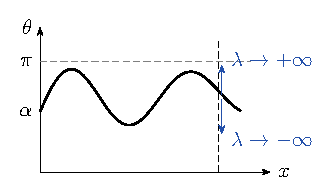
\includegraphics[scale=0.55]{ch05_fig_5_2_1a}\\[0.6em]
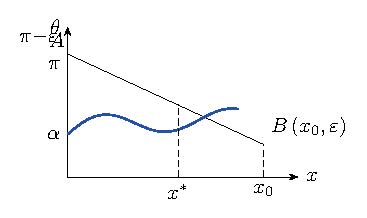
\includegraphics[scale=0.55]{ch05_fig_5_2_1b}
\end{center}

Now for each $k\in\N$ there is $\lambda_k$ s.t.\ $\theta(1,\lambda_k)=\beta+k\pi$; the
$\lambda_k\nearrow+\infty$ and each $\lambda_k$ is unique. This gives all eigenvalues
$\lambda_k$ \& eigenfunctions $\varphi(x,\lambda_k)$. Every eigenspace is 1-dim because the initial
data are linearly dependent $\Rightarrow$ solutions are dependent.

\begin{center}
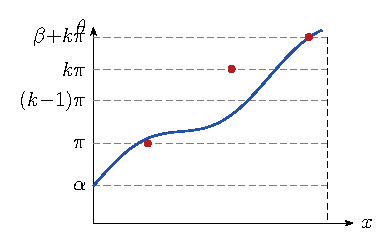
\includegraphics[scale=0.6]{ch05_fig_5_2_2}
\end{center}

\textbf{Zeros.} $\varphi(x^*,\lambda_k)=0\iff\sin\theta(x^*,\lambda_k)=0$. For $k\ge1$ there are $k$
zeros $x_j\in(0,1)$; at a zero,
$\theta'(x_j,\lambda_k)=\cos\theta+(\lambda_kr+q)\sin\theta\equiv1$, so each level $j\pi$ is crossed
only once. For $k=0$, $\theta(x,\lambda_0)=j\pi$ has no solution (checking the sketches for
$\beta=\pi$ and $\beta<\pi$).

\textbf{Oscillation of zeros.} For $\lambda_m>\lambda_n$ we have $\lambda_mr+q>\lambda_nr+q$; by
Sturm comparison, between 2 consecutive zeros of $\varphi(x,\lambda_n)$ there is a zero of
$\varphi(x,\lambda_m)$.

\begin{center}
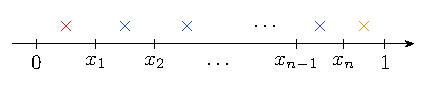
\includegraphics[scale=0.62]{ch05_fig_5_2_3}
\end{center}

For $\varphi(x,\lambda_n)$ \& $\varphi(x,\lambda_{n+1})$, let
$0<x_1<\cdots<x_n<1$ be the zeros of $\varphi(x,\lambda_n)$. In any $(x_k,x_{k+1})$ there is a zero
of $\varphi(x,\lambda_{n+1})$. In $(0,x_1)$: $\theta(x_1,\lambda_{n+1})>\theta(x_1,\lambda_n)=\pi$
while $\theta(0,\lambda_{n+1})=\alpha<\pi$, so there is $x^*\in(0,x_1)$ with
$\theta(x^*,\lambda_{n+1})=\pi$. In $(x_n,1)$: if $\varphi(x,\lambda_{n+1})\ge0$ on $[x_n,1]$, the
proof of Sturm comparison gives a contradiction; so $\exists\, x^{**}\in(x_n,1)$ with
$\varphi(x^{**},\lambda_{n+1})=0$. For orthogonality, notice the $\lambda_k$ are different. \qed

\secn{5.3\quad Periodic Sturm--Liouville problem}

Consider $y''+(\lambda r+q)y=0$, $r,q\in C[0,1]$, $r>0$, with $r,q$ 1-periodic; ask for 1-periodic
solutions.

\textbf{General setting:} $y''=f(x,y,y')$ with $f$ locally Lipschitz in $y,y'$ and 1-periodic in $x$.

\begin{lemma}
Any solution satisfying $y(0)=y(1)$, $y'(0)=y'(1)$ is a 1-periodic solution.

\textbf{Pf.} $y(x+1)$ satisfies the same IVP as $y(x)$. \qed
\end{lemma}

Consider $\mathcal{L}:=\frac{1}{r(x)}\bigl(\frac{d^2}{dx^2}+q(x)\bigr)$, $r>0$, $r,q\in C[0,1]$
1-periodic; $X:=\{f\in C^2[0,1]\}$, $\langle f,g\rangle=\int_0^1r(x)f(x)g(x)\,dx$,
\[
D(\mathcal{L}):=\{f\in X:\ f(0)=f(1)\ \&\ f'(0)=f'(1)\}.
\]
$\mathcal{L}$ is symmetric on $D(\mathcal{L})$; so we study $\mathcal{L}y=-\lambda y$.

\textbf{Special case.} $r\equiv1$, $q\equiv0$.

\begin{theorem}[(Periodic Sturm--Liouville problem)]
\begin{itemize}
\item[(1)] The eigenvalues are countable:
$\lambda_0<\lambda_1\le\lambda_2<\lambda_3\le\lambda_4<\cdots<\lambda_{2k-1}\le\lambda_{2k}<\cdots$.
\item[(2)] $\lambda_0$ has a 1-dim eigenspace.
\item[(3)] If $\lambda_{2k-1}<\lambda_{2k}$, each of them has a 1-dim eigenspace.
\item[(4)] If $\lambda_{2k-1}=\lambda_{2k}=\lambda$, then $\lambda$ has a 2-dim eigenspace.
\item[(5)] $\varphi(x,\lambda_0)$ has no zero in $[0,1)$; $\varphi(x,\lambda_{2k-1})$ \&
$\varphi(x,\lambda_{2k})$ have $2k$ zeros in $[0,1)$.
\item[(6)] Orthogonality \& completeness hold.
\end{itemize}
\end{theorem}

\textbf{Pf.}
\textbf{Step 1 (Foundation): reconstruct the boundary conditions.} Take fundamental solutions
$\begin{pmatrix}\varphi(0)\\ \varphi'(0)\end{pmatrix}=\begin{pmatrix}1\\0\end{pmatrix}$,
$\begin{pmatrix}\psi(0)\\ \psi'(0)\end{pmatrix}=\begin{pmatrix}0\\1\end{pmatrix}$; any solution is
$y=c_1\varphi+c_2\psi$. The boundary conditions give
\[
\begin{pmatrix} 1-\varphi(1,\lambda) & -\psi(1,\lambda)\\ -\varphi'(1,\lambda) & 1-\psi'(1,\lambda) \end{pmatrix}
\begin{pmatrix} c_1\\ c_2 \end{pmatrix}=0,
\qquad
\det A(\lambda)=2-\varphi(1,\lambda)-\psi'(1,\lambda)
\]
(using $W(\varphi,\psi)=1$). Denote $f(\lambda)=\varphi(1,\lambda)+\psi'(1,\lambda)$: $\lambda$ is
an eigenvalue $\iff f(\lambda)=2$. Moreover, $\lambda$ gives 2 independent solutions
$\iff A(\lambda)\equiv0 \iff \varphi(1,\lambda)=1,\ \psi(1,\lambda)=0,\ \varphi'(1,\lambda)=0,\ \psi'(1,\lambda)=1$.

\textbf{Step 2 (Preparation).} For (I) $y''+(\lambda r+q)y=0$, $y(0)=y(1)=0$, the S--L thm gives
$\mu_0<\mu_1<\cdots\to+\infty$ with $\psi(x,\mu_j)$ solving (I). For (II)
$y''+(\lambda r+q)y=0$, $y'(0)=y'(1)=0$, it gives $\nu_0<\nu_1<\cdots\to+\infty$ with
$\varphi(x,\nu_j)$ solving (II).

\textbf{Step 3 (Properties of $f(\lambda)$).}

\begin{lemma}
$\nu_0\le\mu_0$, $f(\nu_0)\ge2$, $f(\mu_{2j+1})\ge2$, $f(\mu_{2j})\le-2$.

\textbf{Pf.} $1=W(\varphi,\psi)(1)=\varphi(1,\lambda)\psi'(1,\lambda)-\varphi'(1,\lambda)\psi(1,\lambda)$.
For $\lambda=\nu_0$: $\varphi'(1,\nu_0)=0 \Rightarrow \varphi(1,\nu_0)\psi'(1,\nu_0)=1$. For
$\lambda=\mu_j$: $\psi(1,\mu_j)=0 \Rightarrow \varphi(1,\mu_j)\psi'(1,\mu_j)=1$, so
\[
f(\mu_{j})=\psi'(1,\mu_{j})+\frac{1}{\psi'(1,\mu_{j})}.
\]
\begin{center}
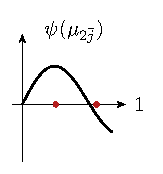
\includegraphics[scale=0.45]{ch05_fig_5_3_1a}\quad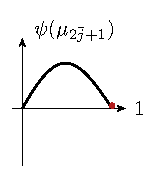
\includegraphics[scale=0.45]{ch05_fig_5_3_1b}
\end{center}
Counting zeros of $\psi(\cdot,\mu_j)$ on $[0,1]$: $\psi'(1,\mu_{2j})<0 \Rightarrow f(\mu_{2j})\le-2$;
$\psi'(1,\mu_{2j+1})>0 \Rightarrow f(\mu_{2j+1})\ge2$. For $\lambda=\nu_0$:
$f(\nu_0)=\varphi(1,\nu_0)+\frac{1}{\varphi(1,\nu_0)}$ with $\varphi(1,\nu_0)>0$, so $f(\nu_0)\ge2$.
If $\nu_0>\mu_0$: $\psi(x,\mu_0)$ has 2 zeros in $[0,1]$, so by comparison $\varphi(x,\nu_0)$ has 1
zero: contradiction. \qed
\end{lemma}

\textbf{Step 4 (Properties of $f'(\lambda)$).} Differentiating the ODEs in $\lambda$: with
$u=\frac{\partial\varphi}{\partial\lambda}$,
$u''+(\lambda r+q)u=-r\varphi$, and using $u(0)=u'(0)=0$,
\[
\frac{\partial}{\partial\lambda}\varphi(1,\lambda)=\int_0^1\bigl(\varphi(1)\psi(s)-\psi(1)\varphi(s)\bigr)r(s)\varphi(s)\,ds,
\qquad
\frac{\partial}{\partial\lambda}\psi'(1,\lambda)=\int_0^1\bigl(\varphi'(1)\psi(s)-\psi'(1)\varphi(s)\bigr)r(s)\psi(s)\,ds.
\]
So
\[
f'(\lambda)=\int_0^1\bigl[a\,\psi^2(s,\lambda)+b\,\psi(s,\lambda)\varphi(s,\lambda)+c\,\varphi^2(s,\lambda)\bigr]r(s)\,ds,
\]
with $a:=\varphi'(1,\lambda)$, $b:=\varphi(1,\lambda)-\psi'(1,\lambda)$, $c:=-\psi(1,\lambda)$.
Notice
\[
b^2-4ac=\varphi^2(1)+\psi'^2(1)-2\varphi(1)\psi'(1)+4\varphi'(1)\psi(1)
=\varphi^2(1)+\psi'^2(1)+2\varphi(1)\psi'(1)-4=(f(\lambda))^2-4.
\]
If $f(\lambda)=2$, then $b^2-4ac=0$; and $-\psi(1,\lambda)\ge0 \Rightarrow f'(\lambda)\ge0$,
$-\psi(1,\lambda)\le0 \Rightarrow f'(\lambda)\le0$, with
$f'(\lambda)=0\iff a,b,c=0\iff A(\lambda)=0$. Hence, for an eigenvalue,
\[
f'(\lambda)=0 \iff \text{the eigenspace of }\lambda\text{ is 2-dim}.
\]
Also, for eigenvalues $\lambda\neq\mu_j$:
$\lambda<\mu_0 \Rightarrow \psi(1,\lambda)>0 \Rightarrow f'(\lambda)<0$;
$\mu_0<\lambda<\mu_1 \Rightarrow f'(\lambda)>0$; and
$\lambda\in(\mu_j,\mu_{j+1}) \Rightarrow f'(\lambda)(-1)^j<0$. Besides, one computes: if
$f(\mu_{2j+1})=2$ and $f'(\mu_{2j+1})=0$, then $f''(\mu_{2j+1})<0$.

\textbf{Step 5 (Existence of eigenvalues).} We have
$\nu_0\le\lambda_0<\mu_0<\lambda_1\le\mu_1\le\lambda_2<\mu_2<\lambda_3\le\mu_3\le\lambda_4$:

\begin{center}
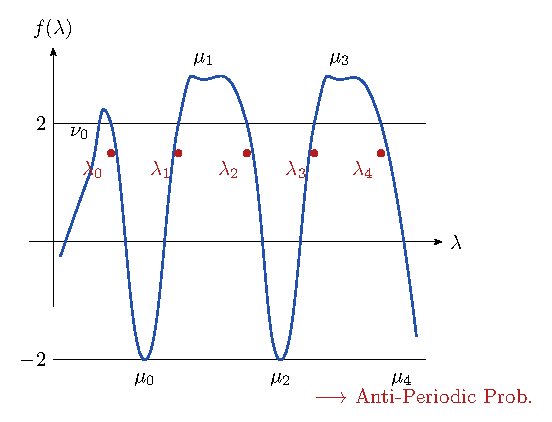
\includegraphics[scale=0.6]{ch05_fig_5_3_2}
\end{center}

\textbf{Case 1.} If $f(\mu_{2j+1})>2$, then
$\lambda_{2j+1}<\mu_{2j+1}<\lambda_{2j+2}<\mu_{2j+2}$, and $\lambda$ is unique in
$(\mu_{2j+1},\mu_{2j+2})$ since $f'\neq0$.

\textbf{Case 2.} If $f(\mu_{2j+1})=2$:

\textbf{Case 2.1} $f'(\mu_{2j+1})\neq0$ (say $>0$): take $\lambda_{2j+1}=\mu_{2j+1}$ and find
$\lambda_{2j+2}\in(\mu_{2j+1},\mu_{2j+2})$, unique with $f'(\lambda_{2j+2})\neq0$; the eigenspace
is 1-dim.

\begin{center}
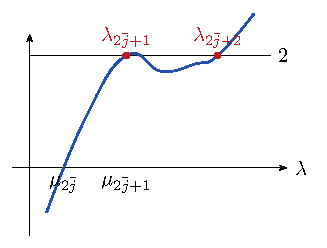
\includegraphics[scale=0.5]{ch05_fig_5_3_3}
\end{center}

\textbf{Case 2.2} $f'(\mu_{2j+1})=0$: $\lambda=\mu_{2j+1}$ has a 2-dim eigenspace; take
$\lambda_{2j+1}=\mu_{2j+1}=\lambda_{2j+2}$, and no other $\lambda$ in
$(\mu_{2j},\mu_{2j+1})\cup(\mu_{2j+1},\mu_{2j+2})$ satisfies $f(\lambda)=2$.

\textbf{Conclusion:} $\lambda_{2j+1}<\lambda_{2j+2} \Rightarrow$ 1-dim eigenspace;
$\lambda_{2j+1}=\lambda_{2j+2} \Rightarrow$ 2-dim eigenspace.

\textbf{Step 6 (Number of zeros).}

\begin{lemma}
If $\lambda$ is an eigenvalue, $\varphi(x,\lambda)$ has an even number of zeros in $[0,1)$.

\textbf{Pf.} Zeros are isolated, hence finite. If $\varphi(0,\lambda)=0$, then
$\varphi(1,\lambda)=0$ and $\varphi'(0,\lambda)=\varphi'(1,\lambda)$; counting gives an even number.
If $\varphi(0,\lambda)\neq0$, same argument. \qed
\end{lemma}

Now $\varphi(x,\lambda_0)$ has no zero in $[0,1)$: otherwise it would have at least 2 zeros, but
$\lambda_0<\mu_0$ and comparison give a contradiction. And $\varphi(x,\lambda_{2j+1})$,
$\varphi(x,\lambda_{2j+2})$ both have $2j+2$ zeros: by comparison with
$\mu_{2j}<\lambda_{2j+1}\le\mu_{2j+1}\le\lambda_{2j+2}<\mu_{2j+2}$ (where $\psi(x,\mu_{2j})$ has
$2j$ zeros, $\psi(x,\mu_{2j+1})$ has $2j+1$, $\psi(x,\mu_{2j+2})$ has $2j+2$), they have between
$2j+1$ and $2j+3$ zeros; being even, both have exactly $2j+2$ zeros in $[0,1)$. \qed

\secn{5.4\quad BVP for nonlinear ODEs}

Consider $\begin{cases} y''=f(x,y,y')\\ y(0)=a,\ y(1)=b \end{cases}$ with $f$ Lipschitz in $y$ \& $y'$.

\subsecn{5.4.1\quad Shooting method}

Solve $\begin{cases} y''=f(x,y,y')\\ y(0)=a,\ y'(0)=s \end{cases} \Rightarrow \varphi(x,s)$; we want
$\varphi(1,s)=b$. Consider $F(s)=\varphi(1,s)-b$ ($s$ is a choice).

\begin{theorem}
If the IVP can be solved on $[0,1]$ and $\exists\ s_1>s_2$ with $F(s_1)F(s_2)<0$, then
$\exists\ s^*$ s.t.\ $\varphi(x,s^*)$ solves the BVP.
\end{theorem}

\begin{example}
$\begin{cases} x''(t)=\arctan x(t),\quad t\in[0,1]\\ x(0)=0,\ x(1)=1. \end{cases}$

For the IVP $x(0)=0$, $x'(0)=\lambda$ the solution $\varphi(x,\lambda)$ exists on $[0,1]$ by the
extension thm. Let $F(\lambda):=\varphi(1,\lambda)-1$. For $\lambda=0$: $x(t)\equiv0$, so
$F(0)=-1<0$. For $\lambda=1$: let $T:=\sup\{t_0\in[0,1]:x(t)\ge0 \text{ on } [0,t_0]\}$; then
$x(t)\ge0$ on $[0,T] \Rightarrow x''\ge0 \Rightarrow x'(t)\ge x'(0)=1$, so
\[
x(t)-x(0)=\int_0^{t}x'(t)\,dt\ge t \quad\Rightarrow\quad x(t)\ge t.
\]
In particular $x(T)\ge T>0$, hence $T=1$; so $x(1)\ge1$, i.e.\ $F(1)\ge0$. There is $\lambda^*$ with
$F(\lambda^*)=0$, giving a solution of the BVP. \qed
\end{example}

\subsecn{5.4.2\quad Periodic BVP}

Consider $\begin{cases} y''=f(x,y,y')\\ y(0)=y(1),\ y'(0)=y'(1) \end{cases}$ with
$f(x+1,\cdot,\cdot)=f(x,\cdot,\cdot)$.

The IVP with $y(0)=\alpha$, $y'(0)=\beta$ gives $\varphi(1,\alpha,\beta)$; we want
$\varphi(1,\alpha,\beta)=\alpha$, $\varphi'(1,\alpha,\beta)=\beta$. The \textbf{Poincar\'e map}
$P(\alpha,\beta)=\bigl(\varphi(1,\alpha,\beta),\ \varphi'(1,\alpha,\beta)\bigr)^{T}$ should have a
\textbf{fixed point}.

\textbf{Methods for finding fixed points:} (1) Banach's fixed point thm.; (2) Brouwer's fixed point
thm.\ (continuous $P:D\to D$ with $D$ compact \& convex); (3) the implicit function thm (locally).

\begin{example}
$x''+\omega_0^2x=p(t)+\varepsilon f(t,x,x')$ with $\omega_0>0$, $\frac{\omega_0}{2\pi}\notin\Z$,
$p$ 1-periodic, $f(t+1,\cdot,\cdot)=f(t,\cdot,\cdot)$. If $\varepsilon$ is small enough, the
equation has a 1-periodic solution.

\textbf{Pf.} For the IVP $x(0)=x_0$, $x'(0)=v_0$ we have the unique solution
$\varphi(x;x_0,v_0,\varepsilon)$; we want
\[
\begin{cases} \varphi(1,x_0,v_0,\varepsilon)=x_0\\ \varphi'(1,x_0,v_0,\varepsilon)=v_0 \end{cases}
\quad\Longleftrightarrow\quad
\begin{cases} F:=\varphi(1,x_0,v_0,\varepsilon)-x_0=0\\ G:=\varphi'(1,x_0,v_0,\varepsilon)-v_0=0. \end{cases}\quad(*)
\]
For $\varepsilon=0$:
\[
x(t,x_0,v_0,0)=x_0\cos\omega_0t+\frac{v_0}{\omega_0}\sin\omega_0t+\frac{1}{\omega_0}\int_0^{t}p(s)\sin\omega_0(t-s)\,ds.
\]
Substituting into $(*)$, the determinant $\Delta\neq0$; so $(*)$ is solved by some $(x_0^*,v_0^*)$.
Since $\frac{\partial(F,G)}{\partial(x_0,v_0)}\big|_{(x_0^*,v_0^*)}=\Delta\neq0$, a vector function
$(x_0(\varepsilon),v_0(\varepsilon))$ exists. By the implicit function thm, in a small neighborhood
of $(x_0^*,v_0^*)$ \& $\varepsilon=0$ there are $x_0(\varepsilon),v_0(\varepsilon)$ with
$F\equiv G\equiv0$, giving a 1-periodic solution for all small $\varepsilon$. \qed
\end{example}

\begin{example}
$x''+x+C\arctan x=\sin t$ with $|C|>\frac12$ has a $2\pi$-periodic solution.

\textbf{Pf.} \textbf{Step 1 (set up).} The homogeneous equation $x''+x=0$ has solutions
$\sin t,\cos t$ with $W(t)=\begin{vmatrix}\sin t & \cos t\\ \cos t & -\sin t\end{vmatrix}=-1$.
Consider the solution $\varphi_b(t)$ with $\varphi_b(0)=0$, $\varphi_b'(0)=b$. Since $-\varphi_b(t)$
satisfies the same IVP, $\varphi_b(t)\equiv-\varphi_b(-t)$; so consider
$f(b)=\varphi_b(\pi)-\varphi_b(-\pi)$.

\textbf{Step 2 (properties of $f(b)$).} By variation of parameters:
\[
\varphi_b(t)=b\sin t+\int_0^{t}\sin(t-s)\bigl[\sin s-C\arctan x(s)\bigr]ds,
\]
so
\[
f(b)=\int_{-\pi}^{\pi}\sin^2s\,ds-C\int_{-\pi}^{\pi}\sin s\,\arctan x(s)\,ds
=\pi-C\int_{-\pi}^{\pi}\sin s\,\arctan x(s)\,ds.
\]
Splitting the last integral,
\[
\int_{-\pi}^{\pi}*=\int_{-\pi}^{-\pi+\varepsilon}+\int_{-\pi+\varepsilon}^{-\varepsilon}+\int_{-\varepsilon}^{\varepsilon}+\int_{\varepsilon}^{\pi-\varepsilon}+\int_{\pi-\varepsilon}^{\pi}
=\int_{-\pi+\varepsilon}^{-\varepsilon}+\int_{\varepsilon}^{\pi-\varepsilon}+O(\varepsilon),
\]
\[
\int_{\varepsilon}^{\pi-\varepsilon}*=\int_{\varepsilon}^{\pi-\varepsilon}\sin s\,\arctan x(s)\,ds=O(s)+\pi\cos\varepsilon,
\]
hence
\[
f(b)=\pi\,(1-2\cos C)+O(\varepsilon).
\]
By the shooting method, we are done. \qed
\end{example}

\end{document}
